\documentclass[12pt, titlepage]{report}
\usepackage{consumer_resource_final}
\graphicspath{{./figures/}}

\begin{document}

We discovered in the previous section that we expect microbial communities where a large syntrophic interaction is observed to have a large consumption rate $\gamma_0$ and a small abundance of consumers at equilibrium $S_0$. It is time to work with feasible microbial communities and investigate their local dynamical stability. In short, we want to investigate the behaviour of systems when their populations (of both resources and microbes) at equilibrium are perturbed.

In the next section we will discover and discuss a special regime of parameters designed to shape more dynamically stable systems. We will then move on to study the dynamical stability of microbial communities by examining the shape of their fully dynamically stable regions, looking in what case feasibility implies dynamical stability and checking how the largest eigenvalue changes with the shape of the consumption-syntrophy network. Finally we will investigate what happens when the number of resources in the community is changed.

\subsection{The quest for dynamical stability}
Section \ref{sec : establish master equation for dynamical stability} establishes the master equation
which solutions govern the dynamical stability of our model. We rewrite it here:
\begin{equation}
\det
\begin{pmatrix}
 -D - \lambda  & \Gamma \\
 \Beta & 0-\lambda
\end{pmatrix} = 0.
\label{eq: master equation eigenvalues jacobian}
\end{equation}
That equation is very difficult to solve for $\lambda$. Our goal now is to find a special regime of parameters where we know dynamical stability is ensured. To achieve this, the first step is to make Eq.\eqref{eq: master equation eigenvalues jacobian} simpler.
In general there are many paths to obtain an approximate version of the dynamics. One of them, for instance, is building an effective Lotka-Volterra model. Although we do not study it here, we explicitly compute it in Section \ref{sec : effective LV system}. We choose here a different way and obtain an exact equation when certain assumptions on the spectrum of the Jacobian can be made.
\subsubsection{Simplifying the master equation}\label{section: non marginal equilibria}
% For now we will concentrate on equilibria that are clearly either stable or unstable\footnote{The case of marginally stable systems, where the maximum eigenvalue is zero, will be covered later.}, \ie:
% \begin{equation}
% \lambda_1 \neq 0.
% \end{equation}
Equation \eqref{eq: master equation eigenvalues jacobian} may be simplified if we assume that:
\begin{equation}
\lambda \neq 0.
\end{equation}
Indeed\footnote{Section \ref{sec : zero part of spectrum} elaborates on when that condition is fulfilled.}, a non-zero $\lambda$ implies
\begin{equation}
\det\left(\lambda \identity{N_S}\right)\neq 0,
\end{equation}
where $\identity{N_S}$ stands for the $N_S \times N_S$ identity matrix. One can use this condition to simplify Eq.\eqref{eq: master equation eigenvalues jacobian} using the properties of block matrices \cite{powell_calculating_2011}:
\begin{equation}
\det
\begin{pmatrix}
  -D - \lambda \identity{N_R}  & \Gamma \\
  \Beta & 0-\lambda \identity{N_S}
\end{pmatrix} =
\det\left(-\lambda \identity{N_S}\right)\det\left(-D- \lambda\identity{N_R}+\frac{1}{\lambda}\Gamma \Beta\right).
\end{equation}
Hence Eq.\eqref{eq: master equation eigenvalues jacobian} becomes:
\begin{equation}
\det\left(\lambda^2 \identity{N_R}+D \lambda-\Gamma \Beta\right)=0. \label{eq: master equation non marginal}
\end{equation}
The complexity here is already reduced because we go from the determinant of a $N_R+N_S$ square matrix to a $N_R$ square matrix. We see from the previous expression that the dynamics is essentially dictated by the $\Gamma \Beta$ $N_R$-dimensional square matrix, which is given by:
\begin{equation}
\left(\Gamma \Beta\right)_{\mu \nu} = \sum_i \Gamma_{\mu i} \Beta_{i \nu} = \sum_i \left(\alpha_{\mu i}-\gamma_{i \mu} R^*_\mu \right)\sigma_{i\nu}\gamma_{i\nu}S^*_i. \label{eq : definition Gamma Beta}
\end{equation}
Using standard properties of determinants, we can rewrite Eq.\eqref{eq: master equation non marginal} as\footnote{We can do this because since $m_\mu > 0$, we know $D$ will always be invertible.}:
\begin{equation}
\det\left(-D^{-1}\right)\det\left(-D^{-1}\lambda^2-\lambda+D^{-1}\Gamma\Beta\right)=0\iff {\det\left(S(\lambda)-\lambda\right)=0} \label{eq: eigenvalue problem S}
\end{equation}
with
\begin{equation}
S(\lambda)=D^{-1}\Gamma\Beta-D^{-1}\lambda^2, \label{eq: equation stability S}
\end{equation}
or, component-wise:
\begin{equation}
S_{\mu \nu} = \frac{1}{D_\mu}\left[\left(\sum_i \Gamma_{\mu i}\Beta_{i \nu}\right) - \lambda^2 \delta_{\mu\nu}\right] \label{eq: definition S component wise}.
\end{equation}
%There are many strategies here to find regimes of stability. One is the so-called ``Reductio ad absurdum'', which is explored later in Methods \ref{subsubsec: reductio ad absurdum}.
\subsubsection{Bound on the eigenvalues of the Jacobian}
In order to find a dynamically stable regime -- \ie conditions on the parameters that will guarantee that $\real{\lambda_1} < 0$ (why this matters is detailed in Section \ref{sec : how to determine local dynamical stability}) -- we need to know more about the eigenvalues of the Jacobian. Our most powerful tool in that quest is the Gerschgorin circle theorem \cite{gerschgorin_uber_1931} which allows us to find a bound on the modulus of every eigenvalue of the Jacobian.
% \begin{proof}
% Let $\lambda \in \sigma(A)$. By the circle theorem, there exists $k \in \left\{1,\dots, N\right\}$ such that :
% \begin{equation}
% \abs{\lambda-A_{kk}} \leq \sum_{j\neq k} \abs{A_{kj}}.
% \end{equation}
% We now use the complex identity:
% \begin{equation}
% \abs{\lambda-A_{kk}} \geq \real{\lambda-A_{kk}} = \real{\lambda}-\real{A_{kk}}.
% \end{equation}
% Equation \eqref{eq: alternative version circle theorem} implies:
% \begin{equation}
% \sum_{j\neq k}\abs{A_{kj}} < - \real{A_{kk}}.
% \end{equation}
% Combining the two previous inequalities yields:
% \begin{equation}
% \real{\lambda}-\real{A_{kk}} \leq \abs{\lambda-A_{kk}} \leq \sum_{j\neq k} \abs{A_{kj}} < -\real{A_{kk}}.
% \end{equation}
% Comparing the RHS and LHS of this inequality yields:
% \begin{equation}
% \real{\lambda} < 0.
% \end{equation}
% \end{proof}
More precisely, Section \ref{sec : find critical radius} shows that:
\begin{equation}
\abs{\lambda} \leq R_C \quad \forall \lambda \in \sigma(J^*), \label{eq: overall bound on lambda}
\end{equation}
where we defined the \define{critical radius} $R_C$ as:
\begin{equation}
R_C \defined \max\left\{\max_i\left\{\sum_\nu \abs{B_{i\nu}}\right\}, \max_\mu\left\{\sum_j \abs{\Gamma_{\mu j}}+D_\mu\right\}\right\}.
\end{equation}
This gives us an estimation of how big the eigenvalues can get: we know that all the eigenvalues \important{have} an absolute value smaller than or equal to the critical radius $R_C$.
The next step is to estimate $R_C$ in terms of metaparameters, so that we can get a qualitative insight on how the eigenvalues change when the metaparameters are changed. Section \ref{sec : estimate critical radius parameters} shows that after a few computations, one finds:
\begin{multline}
R_C \approx \max\left\{ \max_i\left(\deg(G,i)\right) \sigma_0 \gamma_0 S_0 \right., \\
 \left.\max_\mu\left\{\left(\deg(A, \mu)+\deg(G, \mu)\right)\abs{\alpha_0-\gamma_0 R_0}+\frac{l_0+\deg(A,\mu)\alpha_0 S_0}{R_0}\right\}\right\}. \label{eq: estimate R_C metaparameters}
\end{multline}
Note that $R_C$ depends not only on all metaparameters but also on the structure of both $A$ and $G$. In particular, $R_C$ increases when the largest degrees of $A$ or $G$ increase.
% The main factor that will determine $R_C$ (and hence the largest magnitude of any eigenvalue) is the structure of the food consumption matrix.



\subsection{LRI regime}
\subsubsection{Analytical expression}\label{sec : strong LRI regime methods}
The bound on the spectrum of the Jacobian Eq.\eqref{eq: overall bound on lambda} is a step in the right direction to find a dynamically stable regime. It is however not sufficient alone. Once again, the Gerschgorin circle theorem comes to our rescue and allows us to enunciate the following lemma, which puts an upper bound on the real part of the spectrum\footnote{We denote the spectrum of a matrix $M$ with the symbol $\sigma(M)$. } of any square matrix.
\begin{lemma}\label{lemma: lemma Gerschgorin circle}
If a $N-$dimensional square matrix $A$ verifies the equations:
\begin{equation}
\real{A_{ii}} + \sum_{j\neq i} \abs{A_{ij}} < 0, \forall \quad i=1, \dots, N, \label{eq: alternative version circle theorem}
\end{equation}
then $\real{\lambda} < 0 \quad \forall \lambda \in \sigma(A)$.
\end{lemma}
\noindent The interested reader may find its proof in Section \ref{sec : proof of lemma circle}. That lemma plays a pivotal role: combined with the ``Reductio ad absurdum'' strategy described in Section \ref{subsubsec: reductio ad absurdum}, it allows us to get the following theorem.
\paragraph{Strong LRI regime}
\begin{theorem}\label{theorem: strong LRI regime}
Let $p$ be a parameter set with a Jacobian at equilibrium $J^*$. If $0$ is not an eigenvalue of $J^*$ and the equations
\begin{equation}
\left(\Gamma \Beta\right)_{\mu\mu} < - \sum_{\nu \neq \mu } \abs{\left(\Gamma \Beta\right)_{\mu \nu}} - R_C^2 \ \forall \mu, \label{eq: strong LRI regime}
\end{equation}
are verified, then $p$ is dynamically stable.
\end{theorem}
\begin{proof}
We assume
\begin{equation}
\left(\Gamma \Beta\right)_{\mu\mu} < - \sum_{\nu \neq \mu } \abs{\left(\Gamma \Beta\right)_{\mu \nu}} -R_C^2 \ \forall \mu.
\end{equation}
This implies:
\begin{equation}
\left(\Gamma \Beta\right)_{\mu\mu} + R_C^2< - \sum_{\nu \neq \mu } \abs{\left(\Gamma \Beta\right)_{\mu \nu}} \ \forall \mu.
\end{equation}
Using Eq.\eqref{eq: overall bound on lambda} and $\imag{\lambda}^2 \leq \abs{\lambda}^2$, we get:
\begin{equation}
  \left(\Gamma\Beta \right)_{\mu\mu} + \imag{\lambda}^2 < - \sum_{\nu \neq \mu } \abs{\left(\Gamma \Beta\right)_{\mu \nu}} \ \forall \mu. \label{eq: low species bound 1 strong}
\end{equation}
It is not difficult to prove that for any complex number:
\begin{equation}
\imag{c}^2 \geq - \real{c^2} \ \forall c \in \mathbb{C}.
\end{equation}
Using this result and dividing Eq.\eqref{eq: low species bound 1 strong} by\footnote{That step is valid because $D_\mu > 0$, $\forall \mu$.} $D_\mu$, we get:
\begin{equation}
\frac{1}{D_\mu}\left[\left(\sum_i \Gamma_{\mu i} \Beta_{i \mu} \right)-\real{\lambda^2}\right] < - \sum_{\nu \neq \mu } \abs{\frac{\sum_i \Gamma_{\mu i}\Beta_{i\nu}}{D_\mu}} \ \forall \mu. \label{eq : component wise LRI strong}
\end{equation}
Looking at Eq.\eqref{eq: definition S component wise}, we see that Eq.\eqref{eq : component wise LRI strong} is equivalent to:
\begin{equation}
\real{S_{\mu \mu}} + \sum_{\nu \neq \mu} \abs{S_{\mu \nu}} < 0\ \forall \mu.
\end{equation}
Lemma \ref{lemma: lemma Gerschgorin circle} implies that all the eigenvalues of $S(\lambda)$ have a negative real part.
Using the ``Reductio ad absurdum'' reasoning from Section \ref{subsubsec: reductio ad absurdum}, that means that if $\real{\lambda_1} \geq 0 $ in Eq.\eqref{eq: equation stability S} (unstable or marginally stable regime), then $\real{\lambda_1} < 0$, which leads to a contradiction. This then implies that the equilibrium is dynamically stable.
\end{proof}
\noindent Theorem \ref{theorem: strong LRI regime} is a strong statement but it also demands strong constraints on the parameters set, namely $\Gamma\Beta$ must have diagonal elements that are ``very negative'', which imposes severe conditions especially on the $\alpha$ and $\gamma$ matrices. That is why we do not expect to find many parameters sets which would be in such a regime. We need to find another more relaxed regime in which more parameters sets could be.
\paragraph{Weak LRI regime}
Another version of Theorem \ref{theorem: strong LRI regime} can be stated. Its proof is in Section \ref{sec : weak LRI regime}. Its assumptions are less restrictive, but that comes with a price : its statement is weaker.
\begin{theorem}\label{theorem: weak LRI regime}
Let $p$ be a parameter set with a jacobian at equilibrium $J^*$. If $0$ is not an eigenvalue of $J^*$ and the equations
\begin{equation}
\left(\Gamma \Beta\right)_{\mu\mu} < - \sum_{\nu \neq \mu } \abs{\left(\Gamma \Beta\right)_{\mu \nu}} \ \forall \mu,
\end{equation}
are verified, then the real eigenvalues of $J^*$ are negative.
\end{theorem}

\subsubsection{Biological interpretation of the theorems}
We observe that the key feature of both of these regimes is that the diagonal element of the $\Gamma\Beta$ matrix is small compared to the opposite of the sum of the absolute value of the off-diagonal elements. What is the biological interpretation behind this?

 Let us consider two different resources labelled $\nu$ and $\mu$ and a species $i$ (Fig.\ref{fig: LRI scheme}).
\begin{figure}
\centering
\frame{\includegraphics[width=0.5\linewidth]{{LRI_scheme}.pdf}}
\caption{Biomass flux from resource $\nu$ to resource $\mu$ through species $i$.}
\label{fig: LRI scheme}
\end{figure}
 That species consumes an amount of biomass $\gamma_{i\nu}S_i^* R_\nu^*$ from resource $\nu$. Out of this, only $\sigma_{i\nu}\gamma_{i\nu}S_i^*$ is dedicated to the growth of species $i$. However species $i$ contributes through syntrophy \important{to the growth} of resource $\mu$. Indeed, resource $\mu$ receives biomass from species $i$: $(\alpha_{\mu_i}-\gamma_{i\mu}R_\mu^*)S_i^*$. If species $i$ receives less biomass from resource $\nu$, $S_i^*$ will decrease and resource $\mu$ gets less biomass from species $i$. Overall the term:
\begin{equation}
\left(\alpha_{\mu i}-\gamma_{i\mu}R^*_\mu\right) \sigma_{i\nu}\gamma_{i\nu}S_i^*
\end{equation}
can be regarded as the impact of resource $\nu$ on resource $\nu$ through species $i$ (normalized by the abundance of resource $\nu$). If it is positive, when resource $\nu$ increases, resource $\mu$ also increases. However if it is negative resource $\mu$ decreases when resource $\nu$ increases. The total impact of resource $\nu$ on resource $\mu$ is obtained by summing over all the species:
\begin{equation}
\sum_i \left(\alpha_{\mu i}-\gamma_{i\mu}R^*_\mu\right) \sigma_{i\nu}\gamma_{i\nu}S_i^*=(\Gamma\Beta)_{\mu\nu}
\end{equation}
The $\Gamma\Beta$ matrix may then be seen as an \important{effective interaction matrix} between the resources. Coming back to the question initially asked, this means that Theorems \ref{theorem: strong LRI regime} and \ref{theorem: weak LRI regime} correspond to a regime where each resource has a very negative impact on its own growth: this is the reason we call it the \define{low intra-resource interaction} (LRI) regime. It is no surprise that such a regime is dynamically stable: if the growth of a resource encouraged its own growth, any small perturbation could lead to either an asymptotic explosion or decay of resources.

\subsubsection{LRI regimes in terms of metaparameters}
So we found that if a system has parameters that respect Eq.\eqref{eq: strong LRI regime} then it is dynamically stable. A naturally arising question is then to ask % in what measure this is compatible with the feasibility equations Eqs.\eqref{eq : feasibility positive d and m} and \eqref{eq : feasability biomass conservation}.
how that equation is translated in terms of metaparameters -- since our ultimate goal is to find what combination of metaparameters and consumption-syntrophy network $(G,A)$ lead to dynamical stability.
The path is simple : we need to find a metaparameters approximation of the resource interaction matrix $(\Gamma\Beta)_{\mu \nu}$, which will allow us to get such a ``metaparameters-version'' of Eq.\eqref{eq: strong LRI regime} and to know what part of the metaparameters space leads for sure to dynamically stable systems.
Using the metaparameters approximations Eqs.\eqref{eq: metaparameters approximations}, Eq.\eqref{eq : definition Gamma Beta} can be simplified as:
\begin{equation}\label{eq: metaparam approximation GammaBeta}
\left(\Gamma \Beta\right)_{\mu \nu}\approx \sigma_0 \gamma_0 S_0 \left(\alpha_0 \sum_i A_{\mu i}G_{i\nu}-\gamma_0 R_0 \sum_i G_{i\mu}G_{i\nu}\right)\defined \sigma_0 \gamma_0 S_0 \left(\alpha_0 O_{\mu \nu}-\gamma_0R_0 C_{\mu\nu}\right),
\end{equation}
where we defined the \define{syntrophy overlap matrix} $O_{\mu\nu}$ and the \define{consumption overlap matrix} $C_{\mu\nu}$ as:
\begin{equation}
O_{\mu\nu} \defined \left(AG\right)_{\mu \nu} \text{ and } C_{\mu\nu} \defined \left(G^TG\right)_{\mu\nu}.
\end{equation}
The opposite effects of syntrophy and consumption is translated by the opposite sign by the opposite sign these two binary matrices have in Eq.\eqref{eq: definition Gamma Beta}. These matrices essentially build the dynamics of our model and an intuitive understanding of them can be very helpful.
The syntrophy overlap matrix $O_{\mu\nu}$ is defined as:
\begin{equation}
O_{\mu\nu} \defined \sum_k A_{\mu k} G_{k\nu}.
\end{equation}
Although $A$ and $G$ are binary, $O$ does not have to and usually will not be. A given consumer $k$ contributes to $O_{\mu\nu}$ if and only if both $A_{\mu k}$ and $G_{k\nu}$ are non zero, that is if consumer $k$ releases resource $\mu$ \textit{and} consumes resource $\nu$. Hence $O_{\mu\nu}$ essentially tells how many species effectively ``link'' resource $\mu$ to resource $\nu$ through the indirect interaction of the species consumption.
Similarly, the consumption overlap matrix is defined as:
\begin{equation}
C_{\mu\nu}=\sum_k G_{k \mu}G_{k \nu}.
\end{equation}
Like $O$, $C$ usually is not binary. The intuition behind $C_{\mu\nu}$ is straightforward: it counts how many species eat both resource $\mu$ and $\nu$.
%Note that $C_{\mu\nu}=C_{\nu\mu}$ (interesting: hard part comes from the antisymmetric part of S).
We then find a lowerbound for the RHS of Eq.\eqref{eq: strong LRI regime}:
\begin{equation}
-\sum_{\nu\neq\mu}\abs{\Gamma\Beta}_{\mu\nu} \geq - \sum_{\nu \neq \mu} \max_{\nu \neq \mu} \abs{\Gamma\Beta}_{\mu\nu} \geq - \deg\left(\mu, O-C \right) \max_{\nu \neq \mu} \abs{\Gamma\Beta}_{\mu\nu}. \label{eq : RHS LRI in terms of metaparameters}
\end{equation}
Combining Eqs.\eqref{eq : RHS LRI in terms of metaparameters}, \eqref{eq: metaparam approximation GammaBeta} and \eqref{eq: strong LRI regime}, we get an approximative strong LRI regime condition on the metaparameters:
\begin{equation}{
\alpha_0 O_{\mu \mu}-\gamma_0R_0 C_{\mu\mu} \lessapprox - \deg(\mu, O-C) \max_{\nu\neq\mu}\abs{\alpha_0 O_{\mu \nu}-\gamma_0 R_0 C_{\mu\nu}}-\frac{R_C^2}{\sigma_0\gamma_0 S_0} \quad \forall \mu.
}\label{eq: LRI metaparams sufficient}
\end{equation}
The corresponding equation for the weak LRI regime is the same without the $R_C$ term.
Since $R_C$ gets smaller as the largest degree of $G$ decreases (see Eq.\ref{eq: estimate R_C metaparameters}) we only expect systems with a low connectance food consumption adjacency matrix to be able to achieve an LRI state.

% This allows to give a necessary condition on the magnitude of $\alpha_0$. Indeed, since the RHS of the previous equation is negative, we need:
% \begin{equation}
% \alpha_0 O_{\mu \mu}-\gamma_0 R_0 C_{\mu\mu} < 0 \ \forall \mu \implies {\alpha_0 \max_\mu \left\{ \frac{O_{\mu\mu}}{C_{\mu\mu}}  \right\} < \gamma_0 R_0 .} \label{eq: LRI necessary maximum alpha0}
% \end{equation}
% Systems where the maximal ratio of $O_{\mu\mu}$ and $C_{\mu\mu}$ is small will more likely lead to a LRI regime than others. The most favoured systems will be those where $O_{\mu\mu}=0 \ \forall \mu$, \ie systems where no species consumes what it itself produces. In that way we may say that coprophagy tends to destabilize microbial communities.
%
% Combining Eq.\eqref{eq : feasability positivity m} and \eqref{eq: LRI necessary maximum alpha0} gives us a necessary condition on $\alpha_0$ for feasible systems:
% \begin{equation}
% \boxed{
% \alpha_0 \left[\max_\mu \left\{O_{\mu\mu}\right\}-\min_\mu \left\{ \frac{\deg(A,\mu)}{\deg(G,\mu)} \right\} \right] \leq \frac{l_0}{\min_\mu\left(\deg(G,\mu)\right)S_0}}.
% \end{equation}
% Although that equation gives us a necessary condition, it is not sufficient. Eq.\eqref{eq: LRI metaparams sufficient}, on the other hand, is and provides an intuitive way of finding a syntrophy adjacency matrix $A_{\mu i}$ that would put a system with a given consumption adjacency $G_{\mu i}$ in an LRI regime. The following section explains how this can be tried numerically.
Let us recap what we accomplished since the start of this Section: we simplified the Master Equation \eqref{eq: master equation eigenvalues jacobian} from a $N_R+N_S$-dimensional to a $N_R$-dimensional polynomial. We then found with the help of the Gerschgorin circle theorem a condition on the parameters of a system which guarantees its dynamical stability, which we called (strong) LRI regime. Finally we derived the equivalent of that condition in terms of metaparameters (Eq.\ref{eq: LRI metaparams sufficient}). What we would like to do now is to be able to look at that equation and say directly what metaparameters and $(G,A)$ we should choose to obtain paramaters in an LRI configuration. That task is however difficult, mainly because Eq.\eqref{eq: LRI metaparams sufficient} is very complicated and mixes the $A$ and $G$-matrices in a far from trivial way. Our strategy then is to design an algorithm which, for a given set of metaparameters and a consumption matrix $G$, gives us back the syntrophy matrix $A$ such that Eq.\eqref{eq: LRI metaparams sufficient} is as close to being satisfied as possible. We discuss below how this can be achieved.


\subsubsection{Monte Carlo Markov Chain algorithm for the optimal syntrophy matrix} \label{section: methods LRI MC solver}

Given a consumption network $G$ and fixed metaparameters, Eq.\eqref{eq: LRI metaparams sufficient} is more likely satisfied if the syntrophy matrix $A$ is such that the LHS of Eq.\eqref{eq: LRI metaparams sufficient} is minimal and its RHS is maximal:
\begin{itemize}
\item The LHS is minimized if $O_{\mu\mu}=(AG)_{\mu\mu}$ is set to its lowest possible value for every $\mu$, that is zero. Because $(AG)_{\mu\mu}=\sum_{i=1}^{N_S} A_{\mu i} G_{i\mu}$ corresponds to the number of species that both consume and release resource $\mu$, we expect the algorithm to yield $A$-matrices that minimize intraspecific syntrophy.
\item On the other hand, if we neglect the $R_C$ term out of simplicity\footnote{We saw \textit{a posteriori} that this decision may have non negligible consequences. More on that in the following Sections.}, the RHS is maximal if $\alpha_0(AG)_{\mu\nu}\approx\gamma_0R_0 (G^TG)_{\mu\nu} \ \forall \nu\neq\mu$. The sum of the off-diagonal elements of $\abs{\alpha_0 AG-\gamma_0 R_0 G^T G}$ is minimized. This means that outside the diagonal, we should have $\frac{\alpha_0}{\gamma_0 R_0} AG \approx  G^T G$. A direct ecological interpretation is harder to draw. For a couple of different resources $(\mu,\nu)$,  $(AG)_{\mu\nu}=\sum_{i=1}^{N_S} A_{\mu i} G_{i\nu}$ is the number of species that at the same time consume resource $\nu$ and release resource $\mu$ and $(G^TG)_{\mu\nu}=\sum_{i=1}^{N_S} G_{i\mu}G_{i\nu}$ is the number of consumers that eat both $\nu$ and $\mu$.

\end{itemize}
Intuitively, we want an algoritm that finds the syntrophy matrix $A$ such that $AG$ is zero on the diagonal and $AG \approx \frac{\gamma_0R_0}{\alpha_0}G^TG$ outside the diagonal. We inspire ourselves from standard Computational Physics techniques and look at the $A$-matrix we are searching for as the matrix which minimizes an ``energy'' -- which remains to be determined. Considering the problem from that angle allows us to use standard, well-known minimization tools. Namely we choose to find the optimal syntrophy matrix through a Metropolis-Hastings Monte Carlo Markov Chain (MCMC) algorithm, explained in Section \ref{section: methods LRI MC solver}.

But what function $E(G,A)$ should we use as the energy that has to be minimized? Since our goal is to build systems in the LRI regime, we use the simplest and most natural function that is compatible with the intuitively expected characteristics of $A$ explained above (\ie $AG$ is zero on the diagonal and equal to $\frac{\gamma_0 R_0}{\alpha_0} G^TG$ outside of it):
\begin{equation}
E(G,A) \defined \sum_\mu \left( \abs{\alpha_0(AG)_{\mu\mu}} + \sum_{\nu\neq\mu} \abs{(\alpha_0 AG-\gamma_0 R_0 G^TG)_{\mu\nu} }\right). \label{eq: dynamical stability methods LRI MC solver energy definition}
\end{equation}
The energy function and hence the optimal syntrophy adjacency matrix $A$ depend on the ratio $\frac{\alpha_0}{\gamma_0 R_0}$. The most rigorous way to proceed would be to compute the optimal $A$-matrix for each different $\alpha_0$, $\gamma_0$ and $G$ we consider. However, because of the way we explore the metaparameters space, this would be computationally too intense\footnote{Indeed we study about $100$ different $\gamma_0$-values and $10$ $\alpha_0$-values. This means that, \important{for each consumption matrix} $G$, we would have to build at least a thousand optimal syntrophy matrices, so about $100'000$ in total.}. In consequence we assume that the optimal $A$ does not depend too strongly on $\alpha_0$ and we choose one fixed value of $\alpha_0$. We take the theoretical largest feasible syntrophy, which is given by Eq.\eqref{eq : largest feasible alpha0}: $\alpha_0 = \min(1-\sigma_0, \sigma_0) \gamma_0 R_0 N_R$. Because $A$ depends on $\frac{\alpha_0}{\gamma_0 R_0}$, that choice of $\alpha_0$ allows us to obtain a syntrophy matrix $A$ that only depends on\footnote{Technically, $A$ also depends on $N_R$ but $N_R$ is completely determined by the shape of $G$.} $\sigma_0$ and $G$. Because $\sigma_0$ is kept fixed throughout this study, we only need to compute one optimal $A$-matrix for each consumption matrix $G$. Finally, the algorithm we use needs to have the connectance of its output matrix as an input; so we choose that the optimal $A$-matrix has the connectance of $G$. For each consumption matrix $G$, the specific $A$ obtained through that MCMC minimization procedure will be referred to as the ``LRI matrix'' of $G$ or similar expressions.
%This means that the outcome of the algorithm is an optimized $A$ \important{for the largest feasible syntrophy}. Since the expression we have for the largest feasible syntrophy is independent of the $G$ matrix, this choice of $\alpha_0$ provides us a sensible way of comparing different consumption networks.


\subsubsection{Outcome of the MCMC algorithm}
% Methods \ref{section: methods LRI MC solver} explains how we designed an algorithm whose goal is to find, for a given consumption matrix $G$, the syntrophy matrix $A$ that should bring us closer to the satisfaction of Eq.\eqref{eq: strong LRI regime}, which we know is a dynamically stable regime. The shape of the $A$-matrix that is the outcome of the algorithm minimizes the energy $E(G,A)$ (Eq.\ref{eq: dynamical stability methods LRI MC solver energy definition}). Namely, $A$ should have the following properties:
% \begin{itemize}
% \item The sum of the diagonal elements of $AG$ is minimized. Because $(AG)_{\mu\mu}=\sum_{i=1}^{N_S} A_{\mu i} G_{i\mu}$ corresponds to the number of species that both consume and release resource $\mu$, we expect the algorithm to yield $A$-matrices that minimize intraspecific syntrophy.
% \item The sum of the off-diagonal elements of $\abs{\alpha_0 AG-\gamma_0 R_0 G^T G}$ is minimized. This means that outside the diagonal, we should have $\frac{\alpha_0}{\gamma_0 R_0} AG \approx  G^T G$. A direct ecological interpretation is harder to draw. For a couple of different resources $(\mu,\nu)$,  $(AG)_{\mu\nu}=\sum_{i=1}^{N_S} A_{\mu i} G_{i\nu}$ is the number of species that at the same time consume resource $\nu$ and release resource $\mu$ and $(G^TG)_{\mu\nu}=\sum_{i=1}^{N_S} G_{i\mu}G_{i\nu}$ is the number of consumers that eat both $\nu$ and $\mu$. \textbf{TO DO: add something here, transition is a bit rough}
% \end{itemize}
As explained above, the LRI MCMC algorithm should give us a syntrophy matrix that both limits intraspecific syntrophy and such that for every couple of different resources $(\mu, \nu)$, the number of species that consume both $\mu$ and $\nu$ is proportional to the number of species that consume $\mu$ and release $\nu$.
%The proportionality constant, which is the same for all $(\mu, \nu)$ is equal to the ratio of the syntrophy and consumption interactions.
Since the connectance and the dimensions of $A$ are fixed, the number of links of $A$ is already decided and the algorithm simply determines how to optimally distribute them.
Figure \ref{fig: dynamical stability results typical shape of consumption syntrophy LRI algorithm} shows that typically the algorithm will put links in a cell $(\mu,i)$ if $(i, \mu)$ is zero, meaning that not only intraspecific syntrophy tries to be avoided but also species that consume a lot of resources will tend to release few of them and vice-versa.
\begin{figure}
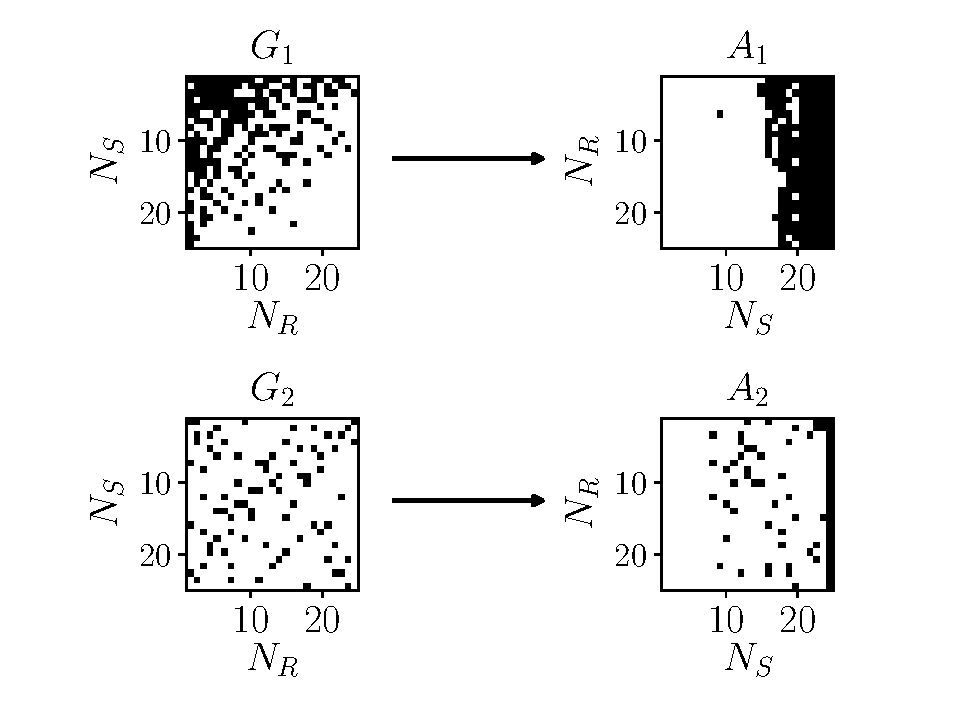
\includegraphics{typical_optimal_LRI_matrix}
\caption{Typical shape of the consumption $G_i$ and syntrophy $A_i$ matrices for $i=1,2$ systems. The white cells symbolize a zero matrix element and the black cells, a one. $A_i$ here is the outcome of the LRI MCMC algorithm described in Section \ref{section: methods LRI MC solver}. The first row has a consumption matrix with $\eta_1=0.6$ and $\kappa_1=0.32$, the algorithm gives rise to a syntrophy matrix with same connectance and ecological overlap $\approx 0.85$. The second row has $G_2$ with $\eta_2=0.1$ and $\kappa_2=0.13$ and the corresponding syntrophy matrix $A_2$ has ecological overlap $\sim 0.42$. We observe that under this optimisation, species that consume few resources end up releasing many and the other way around.}\label{fig: dynamical stability results typical shape of consumption syntrophy LRI algorithm}
\end{figure}

Figure \ref{fig: dynamical stability optimal LRI requirements met} shows that indeed we obtain for a given $G$ matrix a syntrophy matrix $A$ such that the two requirements above are satisfied as best as possible.
\begin{figure}
  \begin{minipage}[c]{0.67\textwidth}
    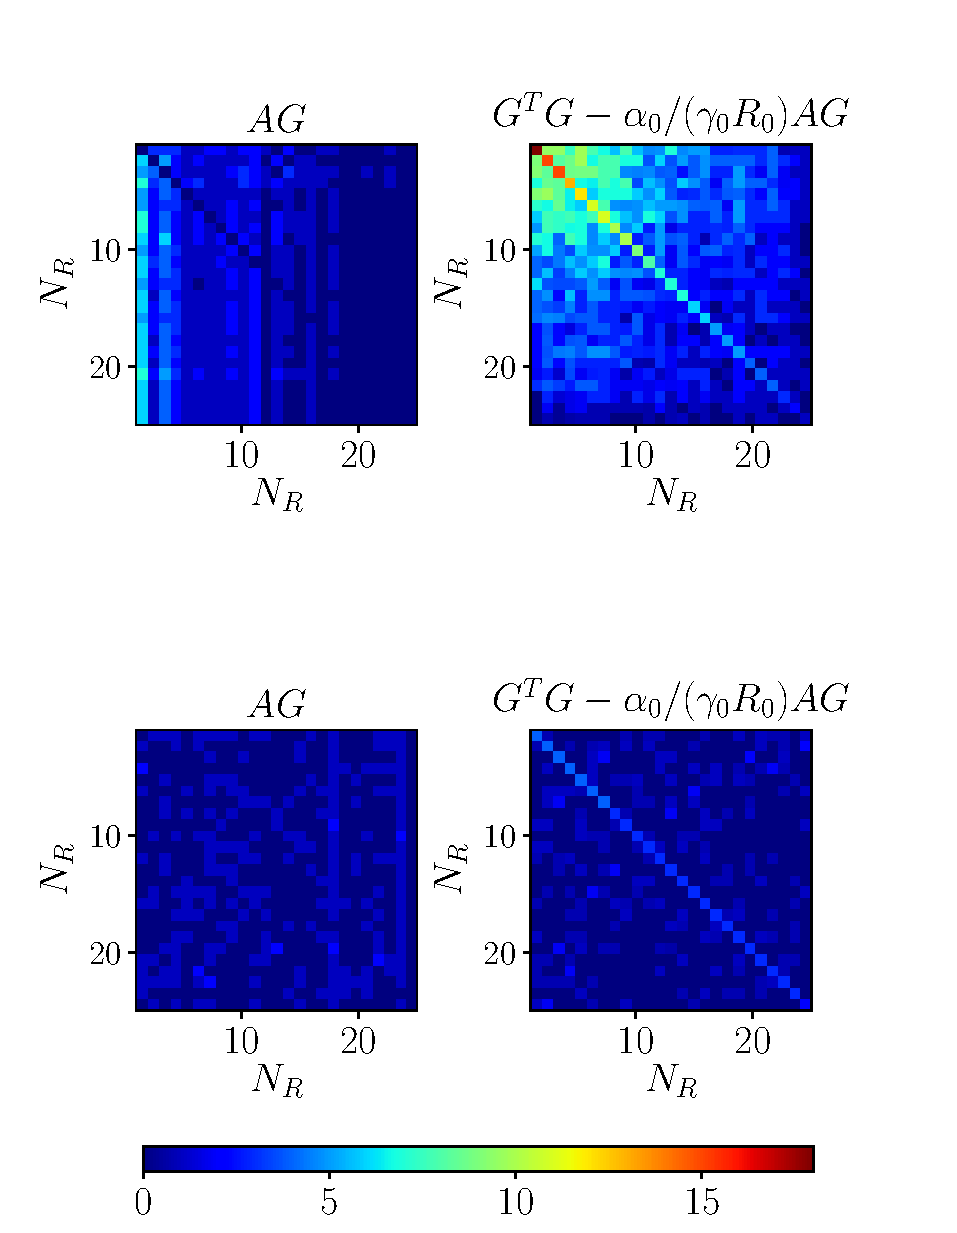
\includegraphics[width=\textwidth]{optimal_LRI_requirements}
  \end{minipage}\hfill
  \begin{minipage}[c]{0.3\textwidth}
    \caption{Plotting of $AG$ and $G^TG-\alpha_0/(\gamma_0R_0) AG$. The $A$ and $G$ matrices of the first and second rows correspond to the respective $A$ and $G$ of Figure \ref{fig: dynamical stability results typical shape of consumption syntrophy LRI algorithm}. As expected, we obtain an $A$ such that intraspecific syntrophy is limited (the diagonal of $AG$ is roughly zero) and, outside the diagonal, $G^TG-\alpha_0/(\gamma_0R_0) AG \approx 0$. The algorithm tries to minimize as much as it can the off-diagonal elements of $G^T G- \alpha_0 /(\gamma_0 R_0 ) AG$, even though this is not always possible (probably because the connectance of $A$ is fixed). Both relations are better satisfied for consumption (and hence syntrophy) matrices with a low connectance.}\label{fig: dynamical stability optimal LRI requirements met}
  \end{minipage}
\end{figure}
As expected, the algorithm works better for matrices with a low connectance.
It is worth noticing that this procedure produces highly nested syntrophy matrices (Fig.\ref{fig: dynamical stability results nestedness LRI outcome}) where only a few species produce most of the syntrophic flow. The obtained matrices have an even larger nestedness if we increase the number of resources.
\begin{figure}
\captionsetup[subfigure]{captionskip = -180pt, margin = 42pt}
\hspace{-0.1\linewidth}
\subfloat[]{\includegraphics[width=0.6\linewidth]{{structure_alpha_matrix_NR25_NS25_with_nestedness}.pdf}}
\subfloat[]{\includegraphics[width=0.6\linewidth]{{structure_alpha_matrix_NR25_N25_with_connectance}.pdf}}

\hspace{-0.1\linewidth}
\subfloat[]{\includegraphics[width=0.6\linewidth]{{structure_alpha_matrix_NR50_NS25_with_nestedness}.pdf}}
\subfloat[]{\includegraphics[width=0.6\linewidth]{{structure_alpha_matrix_NR50_N25_with_connectance}.pdf}}
\caption{Properties of the syntrophy matrix against the consumption matrix in the LRI regime. (a)-(c) Ecological overlap of $A$ as a function of the ecological overlap of $G$ for $N_S=25$ and $N_R=25$ (a) or $N_R=50$ (c). (b)-(d) Ecological overlap of $A$ as a function of the connectance of $G$ for $N_S=25$ and $N_R=25$ (b) or $N_R=50$ (d). The nestedness of the NIS regime is also plotted as a matter of comparison. As $\eta_G$ or $\kappa_G$ increases, the two results will give matrices with similar properties.}
\label{fig: dynamical stability results nestedness LRI outcome}
\end{figure}
\FloatBarrier
\subsection{General considerations}
We observed in Section \ref{sec : feasibility without syntrophy} that, for all $(G,A) \in S_{25}$, at fixed $\alpha_0$ the metaparameters feasibility function $\mathcal{F}\left(m, G, A\right)$ has a typically sharp transition from fully feasible $(\mathcal{F}=1)$ to fully unfeasible ($\mathcal{F}=0$) regimes in the $(\gamma_0, S_0)$ plane. Figure \ref{fig : dynamical stability results typical dynamical stability function} shows that a similar although more complicated behaviour is observed in the case of the dynamical stability function $\mathcal{D}_L\left((\gamma_0, S_0, \alpha_0), G, A\right)$.
\begin{figure}
\captionsetup[subfigure]{captionskip=-225pt, margin=55pt}
\hspace{-0.1\linewidth}
\subfloat[]{\includegraphics[width=1.2\linewidth]{{probability_dynamical_stability_NR25_NS25_Nest0.5_Conn0.416_low_colorbar}.pdf}}

\vspace{-12pt}
\hspace{-0.1\linewidth}
\subfloat[]{\includegraphics[width=1.2\linewidth]{{probability_dynamical_stability_NR25_NS25_Nest0.5_Conn0.416_wo_title_high_colorbar}.pdf}}
%\includegraphics[width=1.2\linewidth]{{probability_dynamical_stability_NR25_NS25_Nest0.5_Conn0.416_wo_title_high_colorbar}.pdf}
\caption{Typical color plot local dynamical stability metaparameters function $\mathcal{D}_L$. for microbial communities with $\eta_G=0.5$ and $\kappa_G=0.42$. The color bar indicates the value of $\mathcal{D}_L\left((\gamma_0, S_0, \alpha_0), G, A\right)$ with $A$ fully connected. Although at first sight, the plane is divided in two zones, one where $\mathcal{D}_L = 0$ and another where $\mathcal{D}_L\approx 1$ (the red and blue regions, respectively, in (a)), upon further notice (b), it turns out the $\mathcal{D}_L \approx 1$ region is very patchy: we observe many $(\gamma_0, S_0, \alpha_0)$ configurations for which $\mathcal{D}_L$ is very close but not exactly equal to $1$. These points are \textit{almost} fully dynamically stable.} \label{fig : dynamical stability results typical dynamical stability function}
\end{figure}
On one hand, the $(\gamma_0, S_0)$ plane is split in two distinct zones, which are also separated by a very narrow boundary. The first zone is characterised by complete dynamical instability, \ie $\mathcal{D}_L =0$. On the other hand, the second zone is not described by full dynamical stability, but rather \important{almost} full dynamical stability: $\mathcal{D}_L$ is very close to but not always exactly equal to 1. The consequence is that the fully dynamically stable region $\mathcal{D}_{L,1}^{G,A}$ will be very patchy.

That patchiness could come from purely numerical effects: $\mathcal{D}_L$ is estimated by generating $N_\text{sys}$ parameters sets and counting the proportion that is dynamically stable, which inevitably leads to an uncertainty on $\mathcal{D}_L$ that could explain the patchiness. This conjecture would hint that most of the points are almost dynamically stable -- for the ones where $\mathcal{D}_L=1$, we simply would not have run enough systems to observe the very rare unstable ones. However that explanation would not justify \important{why} we do not have full dynamical stability.

However, it has been shown for other models \cite{biroli_marginally_2018} that the regime $N_R=N_S$ leads to critical phenomena in communities, which may be linked to ongoing debates about the competitive exclusion principle mentioned above. We here also have the same number of consumers and resources and therefore think that the fact that we observe systems very close to full dynamical stability is an indicator of a similar underlying criticality of our model. That is the reason why we focus our attention on such points.
% In a future project, increasing $N_\text{sys}$ would allow to reduce the relative uncertainty on $\mathcal{D}_L$ and truly discover the origin of this interesting phenomenon.

\subsection{Fully dynamically stable region}\label{sec: dynamical stability methods fully dynamically stable region}
The same way we studied the fully feasible volume $\mathcal{F}_{1}^{G,A}(\alpha_0)$, we investigate now the behaviour of its special subset, the locally fully dynamically stable region $\mathcal{D}^{G,A}_{L,1}\left(\alpha_0\right)$, which is defined\footnote{A formal definition of $\mathcal{D}^{G,A}_{L,1}$ is provided in Section \ref{sec: dynamical stability methods locally dynamically stable region}.} as
\begin{equation}
\mathcal{D}_{L,1}^{G,A}\left(\alpha_0\right) \defined \left\{ (\gamma_0, S_0) : (\gamma_0, S_0, \alpha_0) \in \mathcal{D}^{G,A}_{L,1} \right\}.
\end{equation}
 Intuitively, $\mathcal{D}^{G,A}_{L,1}\left(\alpha_0\right)$ corresponds to the set of all $(\gamma_0, S_0)$ such that $\mathcal{A}\left((\gamma_0, S_0, \alpha_0), G, A\right)$ is a feasible, locally dynamically stable parameters set with probability 1. Since we require $\mathcal{A}\left((\gamma_0, S_0, \alpha_0), G, A\right)$ to be feasible, it is clear that $\mathcal{D}^{G,A}_{L,1}\left(\alpha_0\right)$ is indeed a subset of $\mathcal{F}^{G,A}_1\left(\alpha_0\right)$.

 As a naive approach, one could take a look at the \important{common fully locally dynamically stable region} $\mathcal{D}_{L,1}^{S_{25}}$, which is the intersection of the $\mathcal{D}_{L,1}^{G,A}(\alpha_0) \ \forall (G,A) \in S_{25}$ (Figure \ref{fig: dynamical stability results common fully dynamically stable volume}). However, as said before, because of the patchy and heterogenous nature of each $\mathcal{D}_{L,1}^{G,A}(\alpha_0)$, we observe a very fractured and small common fully locally dynamically stable region, which is the same for all structures of $A$ considered. It has a non-zero volume for $\alpha_0=0$, but for the next point investigated $\alpha_0=\num{1.3e-3}$, no point is fully locally dynamically stable for every matrix considered, which means that the critical common syntrophy is smaller than this. This means that
 %contrarily to the case of feasibility, we must find another, more subtle, approach to study dynamical stability.
 we have to consider each consumption-network individually.
 \begin{figure}
 \hspace{-0.2\linewidth}
 \includegraphics[width=1.4\linewidth]{{common_dynamical_stability_region_NR25_NS25}.pdf}
 \caption{Common full local dynamical stability volume for the four different $A$ structures considered. The points coloured in dark red give rise to locally dynamically stable systems with probability 1 for \important{all the matrices considered}. Very few spots verify this property when there is no syntrophic interaction, and no point gives rise to a fully dynamically stable system for $\alpha_0 = \num{1.3e-3}$. This is independent of the structure of $A$ that we chose. The white points never give rise to fully dynamically stable systems.}\label{fig: dynamical stability results common fully dynamically stable volume}
 \end{figure}


As we saw, $\mathcal{D}_{L,1}^{G,A}\left(\alpha_0\right)$ is geometrically more complex than $\mathcal{F}_{1}^{G,A}\left(\alpha_0\right)$ (Figure \ref{fig: dynamical stability results local dynamical stability region for different matrices}) because of the \important{almost} fully dynamically stable points.
%\footnote{One may argue then that we should also consider the {almost} fully dynamically stable points in the analysis. That position is intellectually appealing but would require to either work in a completely different framework or choose a ``stability threshold'' which separates almost fully feasible points from the others. The arbitrariness of said threshold (should we take into account points above $\mathcal{D}_L=0.99$? Or above $\mathcal{D}_L=0.98$? What about $0.995$?) would make such a point of view hard to hold.}
%(which is after all not suprising, the question of dynamical feasibility is harder than the one of feasibility!)
 It may sometimes have holes, even without syntrophy, and sometimes not, even for matrices that are topologically very close. Compare for instance Fig.\ref{fig: lds region results Nest 0.35 Conn 0.2208} with Fig.\ref{fig: lds region results Nest 0.35 Conn 0.272}, these two networks have the same ecological overlap, but even though their connectance is very similar, their fully locally dynamically stable regions have a very different shape: one of them can sustain only a tiny bit of syntrophy before becoming dynamically unstable (Fig.\ref{fig: lds region results Nest 0.35 Conn 0.2208}) while the second can endure basically any feasible syntrophic interaction (Fig.\ref{fig: lds region results Nest 0.35 Conn 0.272}).

 However, we can still note a general trend among matrices: points with a larger $\gamma_0$ and a smaller $S_0$ tend to remain dynamically stable as shows Figure \ref{fig : dynamical stability results center of stability}. As an aside, note that on this figure the sudden drop of $\av{\gamma_0}_D$ (and rise of $\av{S_0}_D$) at $\alpha_0=\num{9.1e-3}$ is a finite-size effect. Indeed we only monitor points in the unit square $[0,1]^2$, such that the $(G,A)$ for which the center of $\mathcal{D}_{L,1}^{G,A}(\alpha_0)$ leave that zone at $\alpha_0=\num{9.1e-3}$ do not contribute to $(\av{\gamma_0}_D, \av{S_0}_D)$ anymore. Only the $(G,A)$ which previously had a lower, resp. higher, contribution to $\av{\gamma_0}_D$, resp. $\av{S_0}_D$, are taken into account, which results in that strange behaviour. The fact that $\av{\gamma_0}_D$ continues to increase (and $\av{S_0}_D$ to decrease) after that point corroborates that reasoning.

 \begin{figure}
\captionsetup[subfigure]{captionskip = -180pt, margin = 52pt}
%\vspace{-96pt}
\hspace{-0.15\linewidth}
\subfloat[\label{fig: lds region results Nest 0.35 Conn 0.2208}]{\includegraphics[width=1.3\linewidth]{{local_dynamical_stability_wt_wc_region_NR25_NS25_Nest0.35_Conn0.2208}.pdf}}

\vspace{-44pt}
\hspace{-0.15\linewidth}
\subfloat[]{\includegraphics[width=1.3\linewidth]{{local_dynamical_stability_wt_wc_region_NR25_NS25_Nest0.35_Conn0.3216}.pdf}}

\vspace{-44pt}
\hspace{-0.15\linewidth}
\subfloat[\label{fig: lds region results Nest 0.35 Conn 0.272}]{\includegraphics[width=1.3\linewidth]{{local_dynamical_stability_wt_region_NR25_NS25_Nest0.35_Conn0.272}.pdf}}

\caption{Fully locally dynamically stable region $\mathcal{D}_{L,1}^{G,A}$ as a function of syntrophy for different matrices $G$ and the four scenarios of $A$. The white zone corresponds to points that are never fully locally dynamically stable. The colour of a given point tells until which syntrophy that point is fully locally dynamically stable, \eg
a green point is fully locally dynamically stable for $0 \leq \alpha_0 \leq \num{6.5e-3}$. Row (a) corresponds to $G$ with $\eta_G = 0.35$ and $\kappa_G = 0.23$, (b) has $\eta_G=0.35$ and $\kappa_G=0.33$ and (c) $\eta_G=0.35$ and $\kappa_G=0.28$. Even at fixed ecological overlap, different connectances of $G$ give rise to systems which can have very different fully dynamically stable regions.}\label{fig: dynamical stability results local dynamical stability region for different matrices}
\end{figure}


\begin{figure}
\captionsetup[subfigure]{captionskip=-210pt, margin=28pt}
\hspace{-0.1\linewidth}
\subfloat[]{\includegraphics[width=0.6\linewidth]{{local_dynamical_stability_average_gamma0}.pdf}}
\subfloat[]{\includegraphics[width=0.6\linewidth]{{local_dynamical_stability_average_S0}.pdf}}
\caption{(a) Average consumption rate $\av{\gamma_0}_D(\alpha_0)$ and (b) average resource abundance equilibrium
$\av{S_0}_D$ as a function of syntrophy (a formal definition of $(\av{\gamma_0}_D, \av{S_0}_D$ is provided in Section \ref{app : center of gravity local dynamical stability}). Intuitively, $(\av{\gamma_0}_D, \av{S_0}_D$ represents the center $(\gamma_0,S_0)$ point of $\mathcal{D}^{G,A}_{L,1}\left(\alpha_0\right)$,  averaged over all matrices $(G,A) \in S_{25}$, or as we call it the ``\important{center of dynamical stability}''. As syntrophy increases, only points with a large consumption rate and a small resource abundance at equilibrium remain dynamically stable.}\label{fig : dynamical stability results center of stability}
\end{figure}
%We required that a system had to be feasible in order to be dynamically stable, which is the mathematical equivalent of $\mathcal{D}_{L,1}^{G,A}(\alpha_0) \subset \mathcal{F}_1^{G,A}\left(\alpha_0\right)$, \ie local dynamical stability implies feasibility. We may also ask the reverse question, does feasibility imply local dynamical stability?
The question is then: why do other points lose their dynamical stability? Is it because they become unfeasible, or do they remain feasible but become dynamically unstable?
To answer that question, we quantify for each network $(G,A) \in S_{25}$ the \define{probability of being dynamically stable when feasible}, denoted $\text{Prob}\left(\mathcal{D}_L | \mathcal{F}\right)(G,A, \alpha_0)$. That quantity, formally defined in Section \ref{app : probability of being dynamically stable when feasible}, has a straightforward interpretation:
%it computes the average probability over the $(\gamma_0, S_0)$ plane that a $(\gamma_0, S_0, \alpha_0)$ point is dynamically stable if we know it is feasible. In short,
if for a certain $(G,A)$, $\text{Prob}\left(\mathcal{D}_L | \mathcal{F}\right)(G,A, \alpha_0)=x$, then a feasible $(\gamma_0, S_0, \alpha_0)$ has on average a chance $x$ to be dynamically stable\footnote{More precisely, there is a chance $x$ that a parameters set $\mathcal{A}\left((\gamma_0, S_0, \alpha_0), G, A\right)$, which we know is feasible, is also dynamically stable.}. Figure \ref{fig : dynamical stability results proba feas -> dyn sta} shows that $\text{Prob}\left(\mathcal{D}_L | \mathcal{F}\right)(G,A, \alpha_0)< 1$ $\forall (G, A) \in S_{25}$ and $\forall \alpha_0 \geq 0$.
\begin{figure}
%\captionsetup[subfigure]{captionskip=-10}
\hspace{-0.1\linewidth}
\captionsetup[subfigure]{captionskip=-140pt}
\subfloat[]{\includegraphics[width=0.4\linewidth]{{prob_dyn_stab_if_feas_NR25.0_NS25.0_Nest0.5_Conn0.416}.pdf}}
\subfloat[]{\includegraphics[width=0.4\linewidth]{{prob_dyn_stab_if_feas_NR25.0_NS25.0_Nest0.45_Conn0.384}.pdf}}
\subfloat[]{\includegraphics[width=0.4\linewidth]{{prob_dyn_stab_if_feas_NR25.0_NS25.0_Nest0.2_Conn0.0896}.pdf}}

\caption{Plot of the probability that a feasible microbial community is dynamically stable for different consumption-syntrophy networks $(G,A)$. The different lines on the same subplot show the four different $A$-scenarios. The results differ with the consumption matrix considered: (a) $\eta_G=0.5$, $\kappa_G=0.43$, (b) $\eta_G=0.45$, $\kappa_G=0.38$ and (c) $\eta_G=0.2$, $\kappa_G=0.08$. }
\label{fig : dynamical stability results proba feas -> dyn sta}
\end{figure}
That result has a very important biological consequence: there is no consumption-syntrophy network which guarantees that all feasible systems are dynamically stable, \ie there can always exist feasible but dynamically unstable microbial communities\footnote{This does not mean they will survive, of course, since they may vanish at any small perturbation. However it means that there is no physical law that hinders their existence: they can exist, and could appear \eg through mutation processes.}.

%The answer to this is, again, unsurpisingly, ``it depends on the matrix'', as shows Figure \ref{fig: dynamical stability results local dynamical stability region for different matrices}. For instance, for $G$ with $\kappa_G=0.13$ and $\eta_G=0.1$, we have $\text{Vol}\left(\mathcal{D}_{L,1}^{G,A}(\alpha_0)\right) < \text{Vol}\left(\mathcal{F}_{L,1}^{G,A}(\alpha_0)\right) \forall \alpha_0$, which means that for this consumption matrix feasibility does not imply stability. The fully connected case gives a larger dynamically stable volume than the regime without intraspecific syntrophy which is itself better than the LRI regime. This hints that the LRI regime, despite what it was designed for, apparently does not give better results than other structures of $A$.
%On the contrary, for $G$ with $\kappa_G=0.32$ and $\eta_G=0.6$, both volumes are equal at every syntrophy that is feasible, for the three structures of $A$ considered, which shows that for this specific matrix, feasibility implies local dynamical stability.


% A good way to measure how systems react to syntrophy is to compute the \important{critical locally dynamically stable syntrophy} $\alpha_0^D(G,A)$ (see Methods \ref{sec: methods dynamical stability}). An easy way this can be done is by getting some points of the volume of $\mathcal{D}_{L,1}^{G,A}\left(\alpha_0\right)$ curve and finding its intercept to zero. Figure \ref{fig: dynamical stability results typical shrinkage of dynamical volume} shows the typical shrinkage of the fully locally dynamically stable volume.
% To find $\alpha_0^D(G,A)$ for each $G$, we fit with a linear function the last four points of the curve corresponding to Fig.\ref{fig: dynamical stability results typical shrinkage of dynamical volume} and find its intercept to zero $\alpha_0^D(G,A)$. Figure \ref{fig: dynamical stability results critical dynamical syntrophy} shows a very interesting and clear behaviour\footnote{Those results have to be taken with a grain of salt because we did not check whether $\alpha_0^D(G,A)$ was feasible, \ie the actual critical locally dynamically stable syntrophy is the minimum between the value measured in Fig.\ref{fig: dynamical stability results critical dynamical syntrophy} and the largest feasible $\alpha_0$ for that couple $(G,A)$.}: for a given connectance of the consumption matrix, systems that can sustain the largest syntrophy have a small ecological overlap. And for a given ecological overlap, systems with a larger connectance will stay stable longer under the action of syntrophy. In the end, optimal systems have a small ecological overlap and a large connectance: many resources are eaten by the consumers, but they do not share them.

Similarly to what was done for feasibility in Results \ref{sec : feasibility results influence of matrix topology}, we can measure the local dynamical stability volume (see Section \ref{app: how to measure volume}) $\text{Vol}\left(\mathcal{D}_{L,1}^{G,A}(\alpha_0)\right)$ of each consumption-syntrophy network $(G,A)$. $\text{Vol}\left(\mathcal{D}_{L,1}^{G,A}(\alpha_0)\right)$ tells us what proportion of the unit square is occupied by dynamically stable $(\gamma_0, S_0)$ points and is therefore an indicator of how well communities can sustain an increase of average syntrophic strength $\alpha_0$.
Figure \ref{fig: dynamical stability results typical shrinkage of dynamical volume} shows that the dynamically stable volume typically decays in an exponential-like fashion.
\begin{figure}
\hspace{-0.1\linewidth}
\captionsetup[subfigure]{captionskip=-205pt, margin=55pt}
\subfloat[]{\includegraphics[width=0.6\linewidth]{{size_local_dynamical_stability_region_NR25_NS25_Nest0.3_Conn0.2816}.pdf}}
\subfloat[]{\includegraphics[width=0.6\linewidth]{{size_local_dynamical_stability_region_NR25_NS25_Nest0.5_Conn0.416}.pdf}}

\caption{Evolution of the dynamically stable volume $\text{Vol}\left(\mathcal{D}_{L,1}^{G,A}\left(\alpha_0\right)\right)$ (see Section \ref{app: how to measure volume}) with $\alpha_0$ for different $(G,A) \in S_{25}$. (a) $\eta_G=0.3$ and $\kappa_G=0.28$, (b) $\eta_G=0.5$ and $\kappa_G=0.43$. The cross-shaped points indicate the data as measured numerically while the solid lines are the corresponding exponential fit (see main text). The four colors indicate the four $A$-scenarios considered. Independently of the $(G,A)$ network, fewer points are dynamically stable as syntrophy increases.}
\label{fig: dynamical stability results typical shrinkage of dynamical volume}
\end{figure}
We follow the same line of reasoning as Section \ref{sec : feasibility results influence of matrix topology}, and, to quantify that decay, define the \define{dynamical stability decay rate} $d_D(G,A)$ of a consumption-syntrophy network $(G,A)$. It is obtained numerically by finding through a non-linear regression the coefficients $c_1, c_2, d_D \in \mathbb{R}^+$ that satisfy best the relation:
\begin{equation}
\text{Vol}\left(\mathcal{D}_{L,1}^{G,A}(\alpha_0)\right) \approx c_1 \exp\left(-d_D \alpha_0\right)-c_2.
\end{equation}
Much like for the corresponding discussion in the case of feasibility, $d_D(G,A)$ is an indicator of how well a consumption-syntrophy network $(G,A)$ can sustain syntrophy while remaining dynamically stable: a smaller $d_D(G,A)$ indicates a more robust network (it will take a larger syntrophy to find unstable points), a larger $d_D(G,A)$ shows the network is weak against an increase in syntrophic interaction. Figure \ref{fig: dynamical stability results dynamical decay rate FC} shows how $d_D(G,A)$ changes as a function of the characteristics of the consumption matrix $G$, $\forall G \in G_{25}$, when the syntrophy matrix is fully connected.
\begin{figure}
\vspace{-60pt}
\hspace{-0.1\linewidth}
\captionsetup[subfigure]{captionskip=-202pt, margin=42pt}
\subfloat[]{\includegraphics[width=0.6\linewidth]{{local_dynamical_stability_NR25_NS25_dyn_stability_decay_rate_fixed_nestedness_fully_connected}.pdf}}
\subfloat[]{\includegraphics[width=0.6\linewidth]{{local_dynamical_stability_NR25_NS25_dyn_stability_decay_rate_fixed_connectance_fully_connected}.pdf}}
\caption{Dynamical stability decay rate $d_D(G,A)$ for the $A$-matrix fully connected (FC scenario) and every $G \in G_{25}$, (a) as a function of connectance $\kappa_G$ for fixed ecological overlap $\eta_G$ and (b) as a function of ecological overlap for fixed connectance. The trend confirms previous observations: at fixed ecological overlap, a microbial community with a more connected consumption matrix will sustain a larger syntrophy (\ie have a smaller decay rate) and at fixed connectance, systems with a small ecological overlap remain dynamically stable as syntrophy grows.}\label{fig: dynamical stability results dynamical decay rate FC}
\end{figure}
A clear trend may be seen: in order to avoid losing dynamical stability when syntrophy is increased, a microbial community should either increase the number of average resources eaten by each consumer (\ie increase the connectance of the consumption matrix) or decrease its ecological overlap, which means that consumers should stop eating from the same resources. Figure \ref{fig : dynamical stability results decay rate away from FC case} shows how $d_D(G,A)$ changes for each matrix as different syntrophy regimes are considered.
\begin{figure}
\vspace{-35pt}
\captionsetup[subfigure]{captionskip = -188pt, margin = 45pt}
\hspace{-0.05\linewidth}
\subfloat[]{\includegraphics[width=0.55\linewidth]{{local_dynamical_stability_NR25_NS25_dyn_stability_decay_rate_away_from_FC_fixed_nestedness_no_release_when_eat}.pdf}}
\subfloat[]{\includegraphics[width=0.55\linewidth]{{local_dynamical_stability_NR25_NS25_dyn_stability_decay_rate_away_from_FC_syntrophy_fixed_connectance_no_release_when_eat}.pdf}}

\vspace{-12pt}
\hspace{-0.05\linewidth}
\subfloat[]{\includegraphics[width=0.55\linewidth]{{local_dynamical_stability_NR25_NS25_dyn_stability_decay_rate_away_from_FC_fixed_nestedness_optimal_matrix}.pdf}}
\subfloat[]{\includegraphics[width=0.55\linewidth]{{local_dynamical_stability_NR25_NS25_dyn_stability_decay_rate_away_from_FC_syntrophy_fixed_connectance_optimal_matrix}.pdf}}

\vspace{-12pt}
\hspace{-0.05\linewidth}
\subfloat[]{\includegraphics[width=0.55\linewidth]{{local_dynamical_stability_NR25_NS25_dyn_stability_decay_rate_away_from_FC_fixed_nestedness_random_structure}.pdf}}
\subfloat[]{\includegraphics[width=0.55\linewidth]{{local_dynamical_stability_NR25_NS25_dyn_stability_decay_rate_away_from_FC_syntrophy_fixed_connectance_random_structure}.pdf}}

\vspace{-12pt}
%\caption{Relative deviation away from the $FC$ case dynamical stability decay rate as a function of the characteristics of the consumption matrix $G$. A positive $y$-coordinate means that the considered scenario provides a $d_D(G,A)$ smaller than the $FC$ case and is in consequence a sign that the network can better withstand an increase in syntrophy while remaining dynamically stable. We considered the three usual scenarios for the $A$-matrix: (a)-(b) NIS, (c)-(d) LRI and (e)-(f) RS. \textbf{TO DO: compute errors on this graph}}
\caption{Relative difference of the dynamical stability decay rate between the FC scenario and the NIS (Figs. a and b), LRI (c and d) and RS (e and f) scenarios. Positive $y$-values indicate a smoother decay for the considered scenario compared to the FC case. It therefore can sustain higher syntrophy values while remaining dynamically stable.}
\label{fig : dynamical stability results decay rate away from FC case}
\end{figure}
The following comments can be made\footnote{In the following, we use terms like ``is better'', ``outperforms'' or ``improves the dynamical stability'' as a way of saying ``lowers the dynamical stability decay rate compared to the FC case''.}:
\begin{itemize}
\item The NIS scenario slightly lowers the dynamical stability decay rate. It consistently decreases it by $\sim 5-15\%$, except in the case $\kappa_G = 0.18, \eta_G=0.15$, where $d_D(G,A)$ is decreased by $\sim 30\%$.
\item The LRI scenario greatly improves ($> \sim 50\%$) the dynamical stability for consumption matrices with a very low connectance. On average, the lower the connectance, the greater the improvement. However, for larger connectances, it does not change $d_D(G,A)$ in any way.
\item The RS scenario offers the best improvement: any consumption matrix we considered got a considerably better result (at least $>\sim 20 \%$ ). At fixed connectance, the improvement is the same for every ecological overlap considered and the lower the connectance the better the improvement.
\end{itemize}
Overall, dynamical stability follows the same trend as feasibility -- compare the striking similarity between Figure \ref{fig: feasibility results feasibility decay rate vs matrix structure} and \ref{fig : dynamical stability results decay rate away from FC case}. Note that the LRI and RS scenarios offer a more significant improvement the lower the connectance of the consumption matrix. Because both have a syntrophy matrix whose connectance is equal to the one of the consumption matrix, this suggests that microbial communities which have very few syntrophic interactions (\ie $A$ has a low connectance) can remain dynamically stable with a larger average syntrophic interaction than others. Because the random structure (RS) scenario is, for a given matrix, a better improvement than LRI, we think that the syntrophy matrix should also have a lower syntrophic overlap, \ie a low nestedness\footnote{Indeed, the LRI regime has a significantly more nested syntrophy matrix compared to RS (Fig.\ref{fig: dynamical stability results nestedness LRI outcome}). At equal connectance, $A$ with the lower nestedness provides a better improvement.}.


\subsection{Largest eigenvalue of the jacobian} \label{sec: largest eigenvalue of the jacobian}
By studying the very simplified case of a microbial community where both $G$ and $A$ are fully connected and there is no variance in the parameters, we may find after long computations detailed in Section \ref{sec: approximate full spectrum} a condition on the metaparameters that promotes dynamical stability:
\begin{equation}
4N_R \sigma_0 \gamma_0 S_0  (\alpha_0 - \gamma_0 R_0) +\frac{l_0^2}{R_0^2}+\frac{2N_S\alpha_0 S_0 l_0}{R_0^2} + \frac{N_S^2 \alpha_0^2 S_0^2}{R_0^2} \ll 1. \label{eq : dynamical stability methods fully connected metaparameters}
\end{equation}
The smaller the LHS of Eq.\eqref{eq : dynamical stability methods fully connected metaparameters}, the smaller the non-zero real parts of the spectrum of the Jacobian, so the greater the dynamical stability.
Although strictly speaking that relation is only valid for the case where both $G$ and $A$ are fully connected, we expect it to work too when $G$ and $A$ are \important{not too far away} from the fully connected case. It tells us that in order to get more local dynamically stable systems we should\footnote{We do not focus on how $R_0$ and $l_0$ should be changed because they are always equal to $1$ for our study of feasibility and local dynamical stability. }:
\begin{itemize}
  \item Decrease $N_S$ %, $l_0$ \textbf{WEIRD RESULT: would expect that increasing l0 would make systems more dynamically stable (observed in simulations I think)}
  or $\alpha_0$.
  \item If $\alpha_0 - \gamma_0 R_0 < 0$, increase $N _R$, $\sigma_0$ and $\gamma_0$.
  \item Be careful in how $S_0$ is handled: %increasing $S_0$ reduces the $l_0^2/S_0$ term but increases the $N_S^2 \alpha_0^2 S_0$ term. It is very easy to show (Appendix \ref{sec: appendix how to handle S0}) that if $S_0 > l_0/(N_S \alpha_0)$ it should be decreased, and otherwise it should be increased until it reaches $l_0/(N_S \alpha_0)$.
  Section \ref{sec: appendix how to handle S0} shows that at very low syntrophy, we should increase $S_0$ but decrease it when $\alpha_0$ becomes very large. Since in practice the observed feasible $\alpha_0$ are fairly low, we  should increase $S_0$ as much as possible.
\end{itemize}
Combining these considerations with the feasibility conditions Eq.\eqref{eq : fully feasible volume} we expect that -- for all other metaparameters fixed -- systems get more and more locally dynamically stable as $\gamma_0$ is increased and $S_0$ is taken at its largest feasible value. In short, points at the upper border of $\mathcal{D}^{G,A}_{L,1}(\alpha_0)$ should have a lower $\real{\lambda_1}$ as $\gamma_0$ increases. Figure \ref{fig: local dynamical stability results largest eigenvalue} shows that indeed that trend is observed.
\begin{figure}
\hspace{-0.1\linewidth}
\captionsetup[subfigure]{captionskip = -210pt, margin = 26pt}
\subfloat[\label{fig: dynamical stability results typical maximal eigenvalue observed varying syntrophy}]{\includegraphics[width=0.6\linewidth]{{largest_eigenvalue_varying_syntrophy_NR25_NS25_Nest0.3_Conn0.2272}.pdf}}
\subfloat[\label{fig: dynamical stability results shrinkage of DL1G varying syntrophy}]{\includegraphics[width=0.6\linewidth]{{size_local_dynamical_stability_region_NR25_NS25_Nest0.3_Conn0.2272}.pdf}}
\caption{For a consumption matrix $G$ with $\eta_G=0.3$ and $\kappa_G=0.23$. (a) Evolution of the maximal $\abs{\av{\real{\lambda_1}}}$ observed in the $(\gamma_0,S_0) \in [0,1]^2$ region. The maximal eigenvalue increases in magnitude, making the system more dynamically stable, as syntrophy increases. That trend is true for all matrices we considered. (b) Volume of $\mathcal{D}^G_{L,1}(\alpha_0)$. As syntrophy increases, fewer and fewer points become fully dynamically stable. The different structures of the syntrophy matrix are indicated with different colours.}\label{fig: results dynamical stability maximum eigenvalue observed vs size of dynamical region 25x25}
\end{figure}
\begin{figure}
\vspace{-40pt}
\captionsetup[subfigure]{margin=40pt}
\hspace{-0.1\linewidth}
\subfloat[]{\includegraphics[width=1.2\linewidth]{{largest_eigenvalue_wt_NR25_NS25_Nest0.1_Conn0.1296_alpha0=0.0}.pdf}}

\vspace{-12pt}
\hspace{-0.1\linewidth}
\subfloat[]{\includegraphics[width=1.2\linewidth]{{largest_eigenvalue_wt_NR25_NS25_Nest0.1_Conn0.1296_alpha0=0.0039}.pdf}}

\vspace{-12pt}
\hspace{-0.1\linewidth}
\subfloat[]{\includegraphics[width=1.2\linewidth]{{largest_eigenvalue_wt_NR25_NS25_Nest0.1_Conn0.1296_alpha0=0.0078}.pdf}}
\caption{Largest real eigenvalue $\text{Re}(\lambda_1)$ averaged over 200 realisations for each $(\gamma_0, S_0)$ points for the consumption matrix $G$ with consumers overlap $\eta_G = 0.1$ and connectance $\kappa_G=0.13$. The white points correspond to not fully dynamically stable systems. Each row corresponds to a different syntrophy value (a) $\alpha_0 = 0$ (no syntrophic interaction), (b) $\alpha_0 = \num{3.9e-3}$ and (c) $\alpha_0 = \num{7.8e-3}$. The different columns correspond to the different $A$ scenarios considered, which change the shape of the dynamically stable region as seen in the main text. As expected, the boundary points close to the $\gamma_0 \sim S_0^{-1}$ curve are the most stable in every situation. Points with a large $\gamma_0$ are the most stable of the unit square. }\label{fig: local dynamical stability results largest eigenvalue}
\end{figure}
This tells us that if we keep the consumption flux $N_S \gamma_0 S_0$ constant, increasing $\gamma_0$ (and hence decreasing $S_0$) will give rise to more stable systems in the sense that they will recover from changes in the abundance of resources and consumers quicker. Notice that contrarily to the prediction made above, increasing $\alpha_0$ does not decrease stability but increases the maximal $\abs{\real{\lambda_1}}$ observed as shows Fig.\ref{fig: dynamical stability results typical maximal eigenvalue observed varying syntrophy}.

That is coupled with the already discussed shrinkage of the fully locally dynamically stable volume seen on Fig.\ref{fig: dynamical stability results shrinkage of DL1G varying syntrophy}. This means that overall increasing syntrophy makes the system \important{more stable} but at \important{fewer points}. This hints that systems in a high syntrophic regime, where consumers produce a lot of resources, should be very fine tuned and occur for very specific consumption strength and average abundance of consumers.

\FloatBarrier
\subsection{The influence of the matrix dimensions}\label{sec: dyn stab matrix dim}
As said above, because of Eq.\eqref{eq : dynamical stability methods fully connected metaparameters}, we expect dynamical stability to improve when the number of resources is increased and the number of consumers is kept fixed. It is therefore worth briefly studying what happens when the number of resources is doubled $N_R=25 \rightarrow N_R=50$ and every other metaparameter, as well as the number of consumers, keeps the same value as before.

Figure \ref{fig: dynamical stability results typical lds region NR=50 NS=25} shows that the effect of adding resources can be quite dramatic on the stability of the system.
\begin{figure}
\hspace{-0.15\linewidth}
\subfloat[]{\includegraphics[width=1.3\linewidth]{{local_dynamical_stability_region_NR25_NS25_Nest0.45_Conn0.3168}.pdf}}

\hspace{-0.15\linewidth}
\subfloat[]{\includegraphics[width=1.3\linewidth]{{local_dynamical_stability_region_NR50_NS25_Nest0.45_Conn0.3328}.pdf}}
\caption{Fully dynamically stable region $\mathcal{D}^{G,A}_{L,1}$ with the four different structures of $A$ considered. The two matrices considered have the same ecological overlap and connectance, only the number of resources changes. (a) $G$ has $N_R=25$, $N_S=25$ and $\kappa_G=0.33$ and $\eta_G=0.45$. (b) $G$ has $N_R=50$, $N_S=25$ and $\kappa_G=0.33$ and $\eta_G=0.45$.
%(by lack of time, a fewer resolution on the unit square had to be taken)
At $N_R=50$, the typical fully dynamically stable region seems less disconnected. More points can sustain an increased syntrophy for most of the matrices of the set.} \label{fig: dynamical stability results typical lds region NR=50 NS=25}
\end{figure}
For that specific matrix for instance, adding resources allowed for a way larger $\mathcal{D}^{G,A}_{L,1}\left(\alpha_0\right)$ at each $\alpha_0$. This however does not hold for all networks. Figure \ref{fig: dyn stab results dynamical decay rate NR=50 NS=25} shows the difference in dynamical stability decay rates between the case $N_R=50$ and $N_R=25$. Doubling the number of resources has a very different effect on each matrix. On average the ratio between the two decay rates is 1 and it is not clear which parameter of the matrix topology decides whether stability will be improved or not.

\begin{figure}
\vspace{-84pt}
\captionsetup[subfigure]{captionskip=-202pt, margin=45pt}
\hspace{-0.1\linewidth}
\subfloat[]{\includegraphics[width=0.6\linewidth]{{local_dynamical_stability_decay_rate_50_vs_25_fixed_connectance_fully_connected}.pdf}}
\subfloat[]{\includegraphics[width=0.6\linewidth]{{local_dynamical_stability_decay_rate_50_vs_25_fixed_nestedness_fully_connected}.pdf}}

\hspace{-0.1\linewidth}
\subfloat[]{\includegraphics[width=0.6\linewidth]{{local_dynamical_stability_decay_rate_50_vs_25_fixed_connectance_no_release_when_eat}.pdf}}
\subfloat[]{\includegraphics[width=0.6\linewidth]{{local_dynamical_stability_decay_rate_50_vs_25_fixed_nestedness_no_release_when_eat}.pdf}}

\caption{Ratio of the dynamical stability decay rates at $N_R=25$ and at $N_R=50$ as a function of the consumption matrix properties. A $y$-axis larger than $1$ means $d_D(N_R=25)$ is larger than $d_D(N_R=50)$, which means the system remains ``more'' dynamically stable as syntrophic interaction is added at $N_R=50$ compared to $N_R=25$. We considered the four usual $A$ scenarios (a)-(b) FC, (c)-(d) NIS, (e)-(f) LRI and (g)-(h) RS. Increasing the number of resources in the system does not allow microbial communities to be ``more dynamically stable'', on average, as syntrophy increases. Indeed the average ratio between the dynamical stability decay rates is very close to 1.}
\label{fig: dyn stab results dynamical decay rate NR=50 NS=25}
\end{figure}
\begin{figure}
\ContinuedFloat
\captionsetup[subfigure]{captionskip=-202pt, margin=45pt}
\hspace{-0.1\linewidth}
\subfloat[]{\includegraphics[width=0.6\linewidth]{{local_dynamical_stability_decay_rate_50_vs_25_fixed_connectance_optimal_matrix}.pdf}}
\subfloat[]{\includegraphics[width=0.6\linewidth]{{local_dynamical_stability_decay_rate_50_vs_25_fixed_nestedness_optimal_matrix}.pdf}}

\vspace{-12pt}
\hspace{-0.1\linewidth}
\subfloat[]{\includegraphics[width=0.6\linewidth]{{feasibility_decay_rate_50_vs_25_fixed_connectance_random_structure}.pdf}}
\subfloat[]{\includegraphics[width=0.6\linewidth]{{feasibility_decay_rate_50_vs_25_fixed_nestedness_random_structure}.pdf}}

\caption{Continuation of Figure above.}

\end{figure}

We can also observe on Figure \ref{fig: dynamical stability results typical lds region NR=50 NS=25}, that adding more resources seems to take away the patchniness of $\mathcal{D}_{L,1}^{G,A}(\alpha_0)$. We think that this effect happens for all matrices because the common fully locally dynamically stable region has a radically differnt shape. Indeed $\mathcal{D}_{L,1}^{S_{50}}(\alpha_0)$ is smoother than $\mathcal{D}_{L,1}^{S_{25}}(\alpha_0)$ and can sustain a non-zero syntrophy (see the striking difference between Figure \ref{fig: dynamical stability results common fully dynamically stable volume} and Figure \ref{fig: dynamical stability results common lds volume NR=50 NS=25}). Recall that  for $N_R=25$, the critical common syntrophy was between $0$ and $\num{1.3e-3}$. It is greatly improved for $N_R=50$: between $\num{3.9e-3}$ and $\num{5.2e-3}$. This supports the theory stated above that the patchiness of the system of the system observed at $N_R=N_S=25$ is the effect of an underlying criticality that does not appear when the number of resources is larger than the number of consumers.
% \begin{figure}
% \hspace{-0.1\linewidth}
% \captionsetup[subfigure]{captionskip = -212pt, margin = 26pt}
% \subfloat[\label{fig: dynamical stability results typical maximal eigenvalue observed varying syntrophy NR=50}]{\includegraphics[width=0.6\linewidth]{{largest_eigenvalue_varying_syntrophy_NR50_NS25_Nest0.3_Conn0.2296}.pdf}}
% \subfloat[\label{fig: dynamical stability results shrinkage of DL1G varying syntrophy NR=50}]{\includegraphics[width=0.6\linewidth]{{size_local_dynamical_stability_region_NR50_NS25_Nest0.3_Conn0.23}.pdf}}
% \caption{(a) For each $(\gamma_0, S_0)$, we generated 200 parameters sets and computed the average of the largest eigenvalue of the Jacobian $\av{\real{\lambda_1}}(\gamma_0,S_0)$. The figure represents the evolution of the maximal $\av{\real{\lambda_1}}(\gamma_0,S_0)$ among all $(\gamma_0, S_0)$ points in the unit square as a function of syntrophy. (b) Evolution of the local dynamical stability volume, $\text{Vol}\left(\mathcal{D}_{L,1}^{G,A}(\alpha_0)\right)$ as defined in Section \ref{app: how to measure volume}, with syntrophy. The consumption matrix $G$ used for these two plots has $\eta_G=0.3$ and $\kappa_G=0.23$, \ie almost equal properties to the one in Fig.\ref{fig: results dynamical stability maximum eigenvalue observed vs size of dynamical region 25x25}, with the only difference that $N_R=50$ here. Even though the size of $\mathcal{D}_{L,1}^{G,A}$ is smaller, the eigenvalues are larger in magnitude.}
% \end{figure}
\begin{figure}
% \vspace{-84pt}
% \hspace{-0.1\linewidth}
% \subfloat[]{\includegraphics[width=0.6\linewidth]{{common_local_dynamical_stability_volume_NR50_NS25_varying_syntrophy_random_structure}.pdf}}
% \subfloat[]{\includegraphics[width=0.6\linewidth]{{common_local_dynamical_stability_volume_NR50_NS25_varying_syntrophy_no_release_when_eat}.pdf}}
%
% \centering
% \subfloat[]{\includegraphics[width=0.6\linewidth]{{common_local_dynamical_stability_volume_NR50_NS25_varying_syntrophy_optimal_matrix}.pdf}}
\hspace{-0.2\linewidth}
\includegraphics[width=1.4\linewidth]{{common_dynamical_stability_region_NR50_NS25}.pdf}
\caption{Common fully dynamically stable volume of the $S_{50}$ matrix set, which comprises of matrices with dimensions $N_R=50$ and $N_S=25$. This figure is the $N_R=50$ version of Figure \ref{fig: dynamical stability results common fully dynamically stable volume}. At a given syntrophy, we observe a larger zone that is fully dynamically stable for all matrices when the number of resources is doubled.}\label{fig: dynamical stability results common lds volume NR=50 NS=25}
\end{figure}

% Even though more syntrophy can be sustained, it seems that the volume of $\mathcal{D}_{L,1}^{G,A}(\alpha_0)$ is smaller at $N_R=50$ than at $N_R=25$ (compare for  instance Fig.\ref{fig: dynamical stability results shrinkage of DL1G varying syntrophy NR=50} with Fig.\ref{fig: dynamical stability results shrinkage of DL1G varying syntrophy}). This is compensated by the fact that way larger eigenvalues are observed at $N_R=50$: although there are (a bit) fewer equilibrium points, these are more stable (compare Fig.\ref{fig: dynamical stability results typical maximal eigenvalue observed varying syntrophy NR=50} and Fig.\ref{fig: dynamical stability results typical maximal eigenvalue observed varying syntrophy}).
%
% This is a trend that we believe holds for all the matrices considered but a more thorough investigation should be conducted before claiming those results to be absolutely true. Since matrices are individually more locally dynamically stable.
\clearpage
\FloatBarrier
%\documentclass[12pt, titlepage]{report}
\usepackage{consumer_resource_final}
\graphicspath{{./figures/}}

\begin{document}
\begin{figure}
\includegraphics{typical_optimal_LRI_matrix}
\caption{Typical shape of the consumption $G_i$ and syntrophy $A_i$ matrices. The white cells symbolize a zero matrix element and the black cells, a one. $A_i$ here is the outcome of the LRI MC algorithm described in Methods \ref{section: methods LRI MC solver}. The first row has a consumption matrix with $\eta_1=0.6$ and $\kappa_1=0.32$, the LRI MC solver gives rise to a syntrophy matrix with same connectance and ecological overlap $\approx 0.85$. The second row has $G_2$ with $\eta_2=0.1$ and $\kappa_2=0.13$ and the corresponding syntrophy matrix $A_2$ has ecological overlap $\sim 0.42$. We observe that under this optimisation, species that consume few resources end up releasing many and the other way around.}\label{fig: dynamical stability results typical shape of consumption syntrophy LRI algorithm}
\end{figure}
\begin{figure}
  \begin{minipage}[c]{0.67\textwidth}
    \includegraphics[width=\textwidth]{optimal_LRI_requirements}
  \end{minipage}\hfill
  \begin{minipage}[c]{0.3\textwidth}
    \caption{Plotting of $AG$ and $G^TG-\alpha_0/(\gamma_0R_0) AG$. The $A$ and $G$ matrices of the first and second rows correspond to the respective $A$ and $G$ of Figure \ref{fig: dynamical stability results typical shape of consumption syntrophy LRI algorithm}. As expected, we obtain an $A$ such that intraspecific coprophagy is limited (the diagonal of $AG$ is roughly zero) and, outside the diagonal, $G^TG-\alpha_0/(\gamma_0R_0) AG \approx 0$. Both relations are better satisfied for consumption (and hence syntrophy) matrices with a low connectance.}\label{fig: dynamical stability optimal LRI requirements met}
  \end{minipage}
\end{figure}
\begin{figure}
\captionsetup[subfigure]{captionskip = -180pt, margin = 42pt}
\hspace{-0.1\linewidth}
\subfloat[]{\includegraphics[width=0.6\linewidth]{{structure_alpha_matrix_NR25_NS25_with_nestedness}.pdf}}
\subfloat[]{\includegraphics[width=0.6\linewidth]{{structure_alpha_matrix_NR25_N25_with_connectance}.pdf}}

\hspace{-0.1\linewidth}
\subfloat[]{\includegraphics[width=0.6\linewidth]{{structure_alpha_matrix_NR50_NS25_with_nestedness}.pdf}}
\subfloat[]{\includegraphics[width=0.6\linewidth]{{structure_alpha_matrix_NR50_N25_with_connectance}.pdf}}
\caption{Properties of the syntrophy matrix against the consumption matrix. (a)-(c) Ecological overlap of $A$ as a function of the ecological overlap of $G$ for $N_S=25$ and $N_R=25$ (a) or $N_R=50$ (c). (b)-(d) Ecological overlap of $A$ as a function of the connectance of $G$ for $N_S=25$ and $N_R=25$ (b) or $N_R=50$ (d). The nestedness of the ``intraspecific syntrophy restricted'' is also plotted as a matter of comparison. As $\eta_G$ or $\kappa_G$ increase, the two results will without surprise give matrices with similar properties. \textbf{Explain this?}}
\label{fig: dynamical stability results nestedness LRI outcome}
\end{figure}
\begin{figure}
\captionsetup[subfigure]{captionskip=-225pt, margin=55pt}
\hspace{-0.1\linewidth}
\subfloat[]{\includegraphics[width=1.2\linewidth]{{probability_dynamical_stability_NR25_NS25_Nest0.5_Conn0.416_low_colorbar}.pdf}}

\vspace{-12pt}
\hspace{-0.1\linewidth}
\subfloat[]{\includegraphics[width=1.2\linewidth]{{probability_dynamical_stability_NR25_NS25_Nest0.5_Conn0.416_wo_title_high_colorbar}.pdf}}
\caption{Typical color plot local dynamical stability metaparameters function $\mathcal{D}_L$. for microbial communities with $\eta_G=0.5$ and $\kappa_G=0.42$. The color bar indicates the value of $\mathcal{D}_L\left((\gamma_0, S_0, \alpha_0), G, A\right)$ with $A$ fully connected. The plane is divided in two zones, one where $\mathcal{D}_L = 0$ and another where $\mathcal{D}_L\approx 1$ (the red and blue regions, respectively, in (a)). Upon further notice (b), it turns out the $\mathcal{D}_L \approx 1$ region is very patchy: we observe many $(\gamma_0, S_0, \alpha_0)$ configurations for which $\mathcal{D}_L$ is very close but not exactly equal to $1$. These points are \textit{almost} fully dynamically stable.} \label{fig : dynamical stability results typical dynamical stability function}
\end{figure}
\begin{figure}
\vspace{-84pt}
\hspace{-0.1\linewidth}
\includegraphics[width=1.2\linewidth]{{common_dynamical_stability_region_NR25_NS25}.pdf}
\caption{Common full local dynamical stability volume for different $A$ structures: (a) fully connected, (b) no intraspecific syntrophy and (c) LRI algorithm. The points coloured in dark red give rise to locally dynamically stable systems with probability 1 for \important{all the matrices considered}. Very few spots verify this property when there is no syntrophic interaction, and no point gives rise to a fully dynamically stable system for $\alpha_0 = \num{1.3e-3}$. This is independent of the structure of $A$ that we chose. The white points never give rise to fully dynamically stable systems.}\label{fig: dynamical stability results common fully dynamically stable volume}
\end{figure}
\begin{figure}
\captionsetup[subfigure]{captionskip = -180pt, margin = 52pt}
%\vspace{-96pt}
\hspace{-0.15\linewidth}
\subfloat[\label{fig: lds region results Nest 0.35 Conn 0.2208}]{\includegraphics[width=1.3\linewidth]{{local_dynamical_stability_wt_wc_region_NR25_NS25_Nest0.35_Conn0.2208}.pdf}}

\vspace{-44pt}
\hspace{-0.15\linewidth}
\subfloat[]{\includegraphics[width=1.3\linewidth]{{local_dynamical_stability_wt_wc_region_NR25_NS25_Nest0.35_Conn0.3216}.pdf}}

\vspace{-44pt}
\hspace{-0.15\linewidth}
\subfloat[\label{fig: lds region results Nest 0.35 Conn 0.272}]{\includegraphics[width=1.3\linewidth]{{local_dynamical_stability_wt_region_NR25_NS25_Nest0.35_Conn0.272}.pdf}}

\caption{Locally fully dynamically stable region $\mathcal{D}_{L,1}^{G,A}$ as a function of syntrophy for different matrices $G$. The white zone corresponds to points that are never fully locally dynamically stable. The colour of a given point tells until which syntrophy that point is fully locally dynamically stable, \eg
a green point is fully locally dynamically stable for $0 \leq \alpha_0 \leq \num{6.5e-3}$. Row (a) corresponds to $G$ with $\eta_G = 0.35$ and $\kappa_G = 0.23$, (b) has $\eta_G=0.35$ and $\kappa_G=0.33$ and (c) $\eta_G=0.35$ and $\kappa_G=0.27$. Even at fixed ecological overlap, different connectances of $G$ give rise to completely different systems in terms of local dynamical stability.}\label{fig: dynamical stability results local dynamical stability region for different matrices}
\end{figure}

\begin{figure}
\captionsetup[subfigure]{captionskip=-210pt, margin=28pt}
\hspace{-0.1\linewidth}
\subfloat[]{\includegraphics[width=0.6\linewidth]{{local_dynamical_stability_average_gamma0}.pdf}}
\subfloat[]{\includegraphics[width=0.6\linewidth]{{local_dynamical_stability_average_S0}.pdf}}
\caption{(a) Average consumption rate $\av{\gamma_0}_D(\alpha_0)$ and (b) average resource abundance equilibrium
$\av{S_0}_D(\alpha_0)$ as a function of syntrophy (a formal definition of $(\av{\gamma_0}_D(\alpha_0), \av{S_0}_D(\alpha_0))$ is provided in Appendix \ref{app : center of gravity local dynamical stability}). Intuitively, $(\av{\gamma_0}_D(\alpha_0), \av{S_0}_D(\alpha_0))$ represents the center $(\gamma_0,S_0)$ point of $\mathcal{D}^{G,A}_{L,1}\left(\alpha_0\right)$,  averaged over all matrices $(G,A) \in S_{25}$, or as we call it the ``\important{center of dynamical stability}''. As syntrophy increases, only points with a large consumption rate and a small resource abundance at equilibrium remain dynamically stable. The sudden drop of $\av{\gamma_0}_D$ (and rise of $\av{S_0}_D$) at $\alpha_0=\num{9.1e-3}$ is a finite-size effect. Indeed we only monitor points in the unit square $[0,1]^2$, such that the $(G,A)$ for which the center of $\mathcal{D}_{L,1}^{G,A}(\alpha_0)$ leave that zone at $\alpha_0=\num{9.1e-3}$ do not contribute to $(\av{\gamma_0}_D, \av{S_0}_D)$ anymore. Only the $(G,A)$ which previously had a lower, resp. higher, contribution to $\av{\gamma_0}_D$, resp. $\av{S_0}_D$, are taken into account, which results in that strange behaviour. The fact that $\av{\gamma_0}_D$ continues to increase (and $\av{S_0}_D$ to decrease) after that point show that this reasoning is right.}\label{fig : dynamical stability results center of stability}
\end{figure}

% \begin{figure}
% \captionsetup[subfigure]{captionskip = -230pt, margin = 50pt}
% \vspace{-96pt}
% \hspace{-0.1\linewidth}
% \subfloat[]{\includegraphics[width=1.2\linewidth]{{feasibility_vs_lds_NR25_NS25_Nest0.1_Conn0.1296}.pdf}}
%
% \hspace{-0.1\linewidth}
% \subfloat[]{\includegraphics[width=1.2\linewidth]{{feasibility_vs_lds_NR25_NS25_Nest0.6_Conn0.3168}.pdf}}
%
% \caption{Ratio of the size of the fully dynamically stable volume and the fully feasible volume for two consumption matrices $G$ (a) with $\eta_G=0.1$ and $\kappa_G=0.13$, (b) with $\eta_G=0.6$ and $\kappa_G=0.32$. We observe different behaviours for different matrices: for (a) feasibility does not imply local dynamical stability even without syntrophy (it is barely feasible but the ratio is a bit below one for $\alpha_0=0$). On the other hand, for (b) feasibility implies local dynamical stability, indeed both regions have the same volume and since $\mathcal{D}_{L,1}^{G,A}(\alpha_0) \subset \mathcal{F}^{G,A}_1(\alpha_0)$, we conclude that both are equal.}
% \end{figure}
\begin{figure}
%\captionsetup[subfigure]{captionskip=-10}
\hspace{-0.1\linewidth}
\captionsetup[subfigure]{captionskip=-140pt}
\subfloat[]{\includegraphics[width=0.4\linewidth]{{prob_dyn_stab_if_feas_NR25.0_NS25.0_Nest0.5_Conn0.416}.pdf}}
\subfloat[]{\includegraphics[width=0.4\linewidth]{{prob_dyn_stab_if_feas_NR25.0_NS25.0_Nest0.45_Conn0.384}.pdf}}
\subfloat[]{\includegraphics[width=0.4\linewidth]{{prob_dyn_stab_if_feas_NR25.0_NS25.0_Nest0.2_Conn0.0896}.pdf}}

\caption{Plot of the probability that a microbial community is dynamically stable under the assumption that it is feasible for different consumption-syntrophy networks $(G,A)$. The different lines on the same subplot show the four different $A$-scenarios. The results differ with the consumption matrix considered: (a) $\eta_G=0.5$, $\kappa_G=0.43$, (b) $\eta_G=0.45$, $\kappa_G=0.38$ and (c) $\eta_G=0.2$, $\kappa_G=0.08$. }
\label{fig : dynamical stability results proba feas -> dyn sta}
\end{figure}

\begin{figure}
\hspace{-0.1\linewidth}
\captionsetup[subfigure]{captionskip=-205pt, margin=55pt}
\subfloat[]{\includegraphics[width=0.6\linewidth]{{size_local_dynamical_stability_region_NR25_NS25_Nest0.3_Conn0.2816}.pdf}}
\subfloat[]{\includegraphics[width=0.6\linewidth]{{size_local_dynamical_stability_region_NR25_NS25_Nest0.5_Conn0.416}.pdf}}

\caption{Evolution of the dynamically stable volume $\text{Vol}\left(\mathcal{D}_{L,1}^{G,A}\left(\alpha_0\right)\right)$ (see Appendix \ref{app: how to measure volume}) with $\alpha_0$ for different $(G,A) \in S_{25}$. (a) $\eta_G=0.3$ and $\kappa_G=0.28$, (b) $\eta_G=0.5$ and $\kappa_G=0.43$. The cross-shaped points indicate the data as measured numerically while the solid lines are the corresponding exponential fit (see main text). The four colors indicate the four $A$-scenarios considered. Independent of the $(G,A)$ network, fewer points are dynamically stable as syntrophy increases.}
\label{fig: dynamical stability results typical shrinkage of dynamical volume}
\end{figure}
% \begin{figure}
% \captionsetup[subfigure]{captionskip = -185pt, margin = 52pt}
% \vspace{-84pt}
% \hspace{-0.1\linewidth}
% \subfloat[]{\includegraphics[width=0.6\linewidth]{{largest_eigenvalue_NR25_NS25_critical_alpha0_fixed_connectance_random_structure}.pdf}}
% \subfloat[]{\includegraphics[width=0.6\linewidth]{{largest_eigenvalue_NR25_NS25_critical_alpha0_fixed_nestedness_random_structure}.pdf}}
%
% \vspace{-12pt}
% \hspace{-0.1\linewidth}
% \subfloat[]{\includegraphics[width=0.6\linewidth]{{largest_eigenvalue_NR25_NS25_critical_alpha0_fixed_connectance_no_release_when_eat}.pdf}}
% \subfloat[]{\includegraphics[width=0.6\linewidth]{{largest_eigenvalue_NR25_NS25_critical_alpha0_fixed_nestedness_no_release_when_eat}.pdf}}
%
% \vspace{-12pt}
% \hspace{-0.1\linewidth}
% \subfloat[]{\includegraphics[width=0.6\linewidth]{{largest_eigenvalue_NR25_NS25_critical_alpha0_fixed_connectance_optimal_matrix}.pdf}}
% \subfloat[]{\includegraphics[width=0.6\linewidth]{{largest_eigenvalue_NR25_NS25_critical_alpha0_fixed_nestedness_optimal_matrix}.pdf}}
% \vspace{-12pt}
% \caption{Critical syntrophy $\alpha_0^D$, defined as the smallest syntrophy for which we can still find metaparameters that will give rise to fully dynamically stable systems. How $\alpha_0^D$ is estimated is explained in the main text. Errors on $\alpha_0^D$ are not plotted but are at most around $10\%$. (a)(c)(e) Evolution of $\alpha_0^D$ with ecological overlap $\eta$ at different connectance. (b)(d)(f) Evolution of $\alpha_0^D$ with connectance $\kappa$ for different ecological overlap. We observe a strong trend: for a given connectance, $\alpha_0^D$ decreases as ecological overlap increases. Also, for a given ecological overlap, $\alpha_0^D$ increases as connectance is increased.}\label{fig: dynamical stability results critical dynamical syntrophy}
% \end{figure}
\begin{figure}
\vspace{-60pt}
\hspace{-0.1\linewidth}
\captionsetup[subfigure]{captionskip=-202pt, margin=42pt}
\subfloat[]{\includegraphics[width=0.6\linewidth]{{local_dynamical_stability_NR25_NS25_dyn_stability_decay_rate_fixed_nestedness_fully_connected}.pdf}}
\subfloat[]{\includegraphics[width=0.6\linewidth]{{local_dynamical_stability_NR25_NS25_dyn_stability_decay_rate_fixed_connectance_fully_connected}.pdf}}
\caption{Dynamical stability decay rate $d_D(G,A)$ for the $A$-matrix fully connected (FC scenario) and every $G \in G_{25}$, (a) as a function of connectance $\kappa_G$ for fixed ecological overlap $\eta_G$ and (b) as a function of ecological overlap for fixed connectance. The trend confirms the previous observations: at fixed ecological overlap, a microbial community with a more connected consumption matrix will sustain a larger syntrophy (\ie have a smaller decay rate) and at fixed connectance, systems with a small ecological overlap remain dynamically stable as syntrophy grows.}\label{fig: dynamical stability results dynamical decay rate FC}
\end{figure}

\begin{figure}
\vspace{-35pt}
\captionsetup[subfigure]{captionskip = -188pt, margin = 45pt}
\hspace{-0.05\linewidth}
\subfloat[]{\includegraphics[width=0.55\linewidth]{{local_dynamical_stability_NR25_NS25_dyn_stability_decay_rate_away_from_FC_fixed_nestedness_no_release_when_eat}.pdf}}
\subfloat[]{\includegraphics[width=0.55\linewidth]{{local_dynamical_stability_NR25_NS25_dyn_stability_decay_rate_away_from_FC_syntrophy_fixed_connectance_no_release_when_eat}.pdf}}

\vspace{-12pt}
\hspace{-0.05\linewidth}
\subfloat[]{\includegraphics[width=0.55\linewidth]{{local_dynamical_stability_NR25_NS25_dyn_stability_decay_rate_away_from_FC_fixed_nestedness_optimal_matrix}.pdf}}
\subfloat[]{\includegraphics[width=0.55\linewidth]{{local_dynamical_stability_NR25_NS25_dyn_stability_decay_rate_away_from_FC_syntrophy_fixed_connectance_optimal_matrix}.pdf}}

\vspace{-12pt}
\hspace{-0.05\linewidth}
\subfloat[]{\includegraphics[width=0.55\linewidth]{{local_dynamical_stability_NR25_NS25_dyn_stability_decay_rate_away_from_FC_fixed_nestedness_random_structure}.pdf}}
\subfloat[]{\includegraphics[width=0.55\linewidth]{{local_dynamical_stability_NR25_NS25_dyn_stability_decay_rate_away_from_FC_syntrophy_fixed_connectance_random_structure}.pdf}}

\vspace{-12pt}
\caption{Relative deviation away from the $FC$ case dynamical stability decay rate as a function of the characteristics of the consumption matrix $G$. A positive $y$-coordinate means that the considered scenario provides a $d_D(G,A)$ smaller than the $FC$ case and is in consequence a sign that the network can better withstand an increase in syntrophy while remaining dynamically stable. We considered the three usual scenarios for the $A$-matrix: (a)-(b) NIS, (c)-(d) LRI and (e)-(f) RS. \textbf{TO DO: compute errors on this graph}}\label{fig : dynamical stability results decay rate away from FC case}
\end{figure}

% \begin{figure}
% \captionsetup[subfigure]{captionskip = -185pt, margin = 52pt}
% \vspace{-84pt}
% \hspace{-0.1\linewidth}
% \subfloat[]{\includegraphics[width=0.6\linewidth]{{largest_eigenvalue_NR25_NS25_critical_alpha0_fixed_connectance_random_structure}.pdf}}
% \subfloat[]{\includegraphics[width=0.6\linewidth]{{largest_eigenvalue_NR25_NS25_critical_alpha0_fixed_nestedness_random_structure}.pdf}}
%
% \vspace{-12pt}
% \hspace{-0.1\linewidth}
% \subfloat[]{\includegraphics[width=0.6\linewidth]{{largest_eigenvalue_NR25_NS25_critical_alpha0_fixed_connectance_no_release_when_eat}.pdf}}
% \subfloat[]{\includegraphics[width=0.6\linewidth]{{largest_eigenvalue_NR25_NS25_critical_alpha0_fixed_nestedness_no_release_when_eat}.pdf}}
%
% \vspace{-12pt}
% \hspace{-0.1\linewidth}
% \subfloat[]{\includegraphics[width=0.6\linewidth]{{largest_eigenvalue_NR25_NS25_critical_alpha0_fixed_connectance_optimal_matrix}.pdf}}
% \subfloat[]{\includegraphics[width=0.6\linewidth]{{largest_eigenvalue_NR25_NS25_critical_alpha0_fixed_nestedness_optimal_matrix}.pdf}}
% \vspace{-12pt}
% \caption{Critical syntrophy $\alpha_0^D$, defined as the smallest syntrophy for which we can still find metaparameters that will give rise to fully dynamically stable systems. How $\alpha_0^D$ is estimated is explained in the main text. Errors on $\alpha_0^D$ are not plotted but are at most around $10\%$. (a)(c)(e) Evolution of $\alpha_0^D$ with ecological overlap $\eta$ at different connectance. (b)(d)(f) Evolution of $\alpha_0^D$ with connectance $\kappa$ for different ecological overlap. We observe a strong trend: for a given connectance, $\alpha_0^D$ decreases as ecological overlap increases. Also, for a given ecological overlap, $\alpha_0^D$ increases as connectance is increased.}\label{fig: dynamical stability results critical dynamical syntrophy}
% \end{figure}



\begin{figure}
\vspace{-40pt}
\captionsetup[subfigure]{margin=40pt}
\hspace{-0.1\linewidth}
\subfloat[]{\includegraphics[width=1.2\linewidth]{{largest_eigenvalue_wt_NR25_NS25_Nest0.1_Conn0.1296_alpha0=0.0}.pdf}}

\vspace{-12pt}
\hspace{-0.1\linewidth}
\subfloat[]{\includegraphics[width=1.2\linewidth]{{largest_eigenvalue_wt_NR25_NS25_Nest0.1_Conn0.1296_alpha0=0.0039}.pdf}}

\vspace{-12pt}
\hspace{-0.1\linewidth}
\subfloat[]{\includegraphics[width=1.2\linewidth]{{largest_eigenvalue_wt_NR25_NS25_Nest0.1_Conn0.1296_alpha0=0.0078}.pdf}}
\caption{Largest real eigenvalue $\text{Re}(\lambda_1)$ averaged over 300 \textbf{TO DO : check number} realisations for each $(\gamma_0, S_0)$ points for the consumption matrix $G$ with consumers overlap $\eta_G = 0.1$ and connectance $\kappa_G=0.13$. The white points correspond to not fully dynamically stable systems. Each row corresponds to a different syntrophy value (a) $\alpha_0 = 0$ (no syntrophic interaction), (b) $\alpha_0 = \num{3.9e-3}$ and (c) $\alpha_0 = \num{7.8e-3}$. The different columns correspond to the different $A$ scenarios considered, which change the shape of the dynamically stable region as seen in the main text. As expected, the boundary points close to the $\gamma_0 \sim S_0^{-1}$ curve are the most stable in every situation. Points with a large $\gamma_0$ are the most stable of the unit square. }\label{fig: local dynamical stability results largest eigenvalue}
\end{figure}

\begin{figure}
\hspace{-0.1\linewidth}
\captionsetup[subfigure]{captionskip = -210pt, margin = 26pt}
\subfloat[\label{fig: dynamical stability results typical maximal eigenvalue observed varying syntrophy}]{\includegraphics[width=0.6\linewidth]{{largest_eigenvalue_varying_syntrophy_NR25_NS25_Nest0.3_Conn0.2272}.pdf}}
\subfloat[\label{fig: dynamical stability results shrinkage of DL1G varying syntrophy}]{\includegraphics[width=0.6\linewidth]{{size_local_dynamical_stability_region_NR25_NS25_Nest0.3_Conn0.2272}.pdf}}
\caption{For a consumption matrix $G$ with $\eta_G=0.3$ and $\kappa_G=0.23$. (a) Evolution of the maximal $\abs{\av{\real{\lambda_1}}}$ observed in the $(\gamma_0,S_0) \in [0,1]^2$ region. The maximal eigenvalue increases in magnitude, making the system more dynamically stable, as syntrophy increases. That trend is true for all matrices we considered. (b) Volume of $\mathcal{D}^G_{L,1}(\alpha_0)$. As syntrophy increases, fewer and fewer points become fully dynamically stable. For both figures, the different lines show the different stand for the different structure of the syntrophy matrix that we considered. \textbf{TO DO: replace this with average version}}\label{fig: results dynamical stability maximum eigenvalue observed vs size of dynamical region 25x25}
\end{figure}

\begin{figure}
\hspace{-0.15\linewidth}
\subfloat[]{\includegraphics[width=1.3\linewidth]{{local_dynamical_stability_region_NR25_NS25_Nest0.45_Conn0.3168}.pdf}}

\subfloat[]{\includegraphics[width=\linewidth]{{local_dynamical_stability_region_NR50_NS25_Nest0.45_Conn0.3328}.pdf}}
\caption{Fully dynamically stable region $\mathcal{D}^{G,A}_{L,1}$ with the three different structures of $A$ considered: fully connected (left), no intraspecific syntrophy (middle) and LRI matrix (right). The two matrices have the same ecological overlap and connectance, only the number of resources changes. (a) $G$ has $N_R=25$, $N_S=25$ and $\kappa_G=0.32$ and $\eta_G=0.45$. (b) $G$ has $N_R=50$, $N_S=25$ and $\kappa_G=0.33$ and $\eta_G=0.45$ (by lack of time, a fewer resolution on the unit square had to be taken). At $NR=50$, the fully dynamically stable region seems less fractured. The fact that more points can sustain an increased syntrophy is a trend for most of the matrices of the set. \textbf{still check this: the others are more less the same or a tad less}.} \label{fig: dynamical stability results typical lds region NR=50 NS=25}
\end{figure}
\begin{figure}
\hspace{-0.1\linewidth}
\captionsetup[subfigure]{captionskip = -210pt, margin = 26pt}
\subfloat[\label{fig: dynamical stability results typical maximal eigenvalue observed varying syntrophy NR=50}]{\includegraphics[width=0.6\linewidth]{{largest_eigenvalue_varying_syntrophy_NR50_NS25_Nest0.3_Conn0.2296}.pdf}}
\subfloat[\label{fig: dynamical stability results shrinkage of DL1G varying syntrophy NR=50}]{\includegraphics[width=0.6\linewidth]{{size_local_dynamical_stability_region_NR50_NS25_Nest0.3_Conn0.2296}.pdf}}
\caption{To be compared with Fig.\ref{fig: results dynamical stability maximum eigenvalue observed vs size of dynamical region 25x25}. The consumption matrix $G$ considered here has $\eta_G=0.3$ and $\kappa_G=0.23$. (a) Maximal average $\abs{\real{\lambda_1}}$ observed in the unit square. (b) Percentage of the unit square occupied by the fully dynamically stable region of $G$ as a function of syntrophy. The matrix considered has almost equal properties to the one in Fig.\ref{fig: results dynamical stability maximum eigenvalue observed vs size of dynamical region 25x25}, with the only difference that $N_R=50$ here. Even though the size of $\mathcal{D}_{L,1}^{G,A}$ is smaller, the eigenvalues are larger in magnitude.}
\end{figure}

% \begin{figure}
% \vspace{-72pt}
% \hspace{-0.0\linewidth}
% \subfloat[]{\includegraphics[width=\linewidth]{{largest_eigenvalue_wt_NR50_NS25_Nest0.1_Conn0.0832_alpha0=0.0}.pdf}}
%
% \vspace{-26pt}
% \hspace{-0.0\linewidth}
% \subfloat[]{\includegraphics[width=\linewidth]{{largest_eigenvalue_wt_NR50_NS25_Nest0.1_Conn0.0832_alpha0=0.0013}.pdf}}
%
% \vspace{-26pt}
% \hspace{-0.0\linewidth}
% \subfloat[]{\includegraphics[width=\linewidth]{{largest_eigenvalue_wt_NR50_NS25_Nest0.1_Conn0.0832_alpha0=0.0039}.pdf}}
% \caption{To be compared with \ref{fig: local dynamical stability results largest eigenvalue} \textbf{Is it really fair? No comparison because connectance is overall quite different and we saw that changing connectance can have quite a dramatic effect}, the zone is smaller but more stable (by a lot) can we really say this?.}\label{fig: dynamical stability results largest eigenvalue NR=50 NS=25}
% \end{figure}

\begin{figure}
\vspace{-84pt}
\hspace{-0.1\linewidth}
\subfloat[]{\includegraphics[width=0.6\linewidth]{{common_local_dynamical_stability_volume_NR50_NS25_varying_syntrophy_random_structure}.pdf}}
\subfloat[]{\includegraphics[width=0.6\linewidth]{{common_local_dynamical_stability_volume_NR50_NS25_varying_syntrophy_no_release_when_eat}.pdf}}

\centering
\subfloat[]{\includegraphics[width=0.6\linewidth]{{common_local_dynamical_stability_volume_NR50_NS25_varying_syntrophy_optimal_matrix}.pdf}}
\caption{Common fully dynamically stable volume. It is larger with a larger number of resources -> even though individually it is not always better, it is better for the worse matrices (since the common volume can handle more syntrophy)}\label{fig: dynamical stability results common lds volume NR=50 NS=25}
\end{figure}

\begin{figure}
\vspace{-84pt}
\captionsetup[subfigure]{captionskip=-202pt, margin=45pt}
\hspace{-0.1\linewidth}
\subfloat[]{\includegraphics[width=0.6\linewidth]{{local_dynamical_stability_decay_rate_50_vs_25_fixed_connectance_fully_connected}.pdf}}
\subfloat[]{\includegraphics[width=0.6\linewidth]{{local_dynamical_stability_decay_rate_50_vs_25_fixed_nestedness_fully_connected}.pdf}}

\hspace{-0.1\linewidth}
\subfloat[]{\includegraphics[width=0.6\linewidth]{{local_dynamical_stability_decay_rate_50_vs_25_fixed_connectance_no_release_when_eat}.pdf}}
\subfloat[]{\includegraphics[width=0.6\linewidth]{{local_dynamical_stability_decay_rate_50_vs_25_fixed_nestedness_no_release_when_eat}.pdf}}

\hspace{-0.1\linewidth}
\subfloat[]{\includegraphics[width=0.6\linewidth]{{local_dynamical_stability_decay_rate_50_vs_25_fixed_connectance_optimal_matrix}.pdf}}
\subfloat[]{\includegraphics[width=0.6\linewidth]{{local_dynamical_stability_decay_rate_50_vs_25_fixed_nestedness_optimal_matrix}.pdf}}

\vspace{-12pt}
\hspace{-0.1\linewidth}
% \subfloat[]{\includegraphics[width=0.6\linewidth]{{feasibility_decay_rate_50_vs_25_fixed_connectancerandom_structure}.pdf}}
% \subfloat[]{\includegraphics[width=0.6\linewidth]{{feasibility_decay_rate_50_vs_25_fixed_nestednessrandom_structure}.pdf}}

\caption{Ratio of the dynamical stability decay rates at $N_R=25$ and at $N_R=50$ as a function of the consumption matrix properties. A $y$-axis larger than $1$ means $d_D(N_R=25)$ is larger than $d_D(N_R=50)$, which means the system remains ``more'' dynamically stable as syntrophic interaction is added at $N_R=50$ compared to $N_R=25$. We considered the four usual $A$ scenarios (a)-(b) FC, (c)-(d) NIS, (e)-(f) LRI and (g)-(h) RS. On average increasing the number of resources in the system does not particularly allow microbial communities to be slightly ``more dynamically stable'' as syntrophy increases since the average ratio between the dynamical stability decay rates is very close to 1. A detailed on how the consumption matrix properties, at least connectance and ecological overlap, or the $A$-scenario precisely modify the improvement is difficult to draw from this data. \textbf{TO DO: put also the one for random structure}}
\label{fig: feasibility results feasibility decay rate NR=50 NS=25}
\end{figure}
\end{document}


\end{document}








\end{document}
